\documentclass[journal=jpcbfk,manuscript=article]{achemso}

\usepackage{graphicx}
\usepackage{wrapfig}
\usepackage{subcaption}
\usepackage{amsmath} % or simply amstext
\usepackage{amssymb}
\usepackage{array}
\usepackage{siunitx}
\usepackage{booktabs}
\usepackage[export]{adjustbox}
\newcommand{\angstrom}{\textup{\AA}}
\newcommand{\colormap}{jet}  % colorbar to use
\usepackage{cleveref}
\usepackage{booktabs}
\usepackage{gensymb}
\usepackage{float}
\usepackage{xr}
\usepackage{tcolorbox}
\usepackage{multicol}

\SectionNumbersOn
%\definecolor{amber}{rgb}{1.0, 0.75, 0.0} % amber
%\definecolor{amber}{rgb}{1.0, 0.84, 0.0} % gold
\definecolor{amber}{rgb}{0.99, 0.76, 0.0} % golden poppy

\externaldocument[S-]{Supporting_Information}

\title{Chemically Selective Transport in a Cross-linked H\textsubscript{II} Phase Lyotropic Liquid Crystal Membrane}
\author{Benjamin J. Coscia}
\affiliation{Department of Chemical and Biological Engineering, University of Colorado Boulder, Boulder, CO 80309, USA}
\author{Michael R. Shirts}
\email{michael.shirts@colorado.edu}
\affiliation{Department of Chemical and Biological Engineering, University of Colorado Boulder, Boulder, CO 80309, USA}

% MRS2: I think it would be useful to have a picture of the pores to 
% allow people to visualize what was going on. ToC might be good, 
% but I think that as people read, they need to see the 3D picture 
% as well to think through things.

\begin{document}

  \graphicspath{{./figures/}}
  
  \begin{abstract}

  The uniform size and complex chemical topology of the pores formed by
  self-assembled amphiphilic molecules such as liquid crystals make them
  promising candidates for selective separations.
  %that 
  %constitute cross-linked inverted hexagonal (H\textsubscript{II})
  %phase lyotropic liquid crystal (LLC) membranes make them promising
  %candidates for selective separation membranes. 
  %MRS3: I do worry that the above makes it look like we are not acknowledging
  %the formulation problems.  Maybe something like: ''models of how chemically
  %selective separation membranes could can function''?  So the focus is more
  %on the science that these membranes could reveal, rather than saying they
  %are good membranes now?  Then we talk about new membranes at the end of the
  %introduction. Thoughts? I didn't go ahead and make  the change since it
  %needs a bit more thought.  I'm open to other ways to reformulate.  Some of
  %this thinking will percolate into the rest of the introduction as well.
  In this work, we observe transport of water, sodium ions and 20 small polar
  solutes within the pores of a lyotropic liquid crystal (LLC) membrane using
  atomistic molecular simulations. We find that the transport of a species is
  dependent not only on molecular size, but on chemical functionality as well.
  The membrane's inhomogeneous composition gives rise to radially dependent
  transport mechanisms with respect to the pore centers. We observe that all
  solutes perform intermittent hops between lengthy periods of entrapment. Three
  different trapping mechanisms are responsible for this behavior. First, solutes
  that drift out of the pore can become entangled among the dense monomer tails.
  Second, solutes can donate hydrogen bonds to the monomer head groups. Third,
  solutes can coordinate with sodium counter ions.  The degree to which a solute
  is affected by each mechanism is dependent on the chemical functionality of the
  solute. Using the insights developed in this study, we can begin to think about
  how to redesign existing LLC membranes in order to perform solute-specific
  separations.
   
  \end{abstract}

  \section{Introduction}

  Membranes capable of separating nm-sized solutes with high selectivity and
  permeability are highly desirable for a number of applications. For example,
  separation of salt from seawater or other briny sources can yield potable
  drinking water.~\cite{fritzmann_state---art_2007} Removal of organic
  micropollutants, such as personal care products, pesticides and
  pharmaceuticals, from surface and groundwaters, can have large benefits for
  public health.~\cite{schwarzenbach_challenge_2006} Finally, one can purify and
  recover dissolved species present in complex hydraulic fracturing flowback
  water waste streams which would help mitigate the effects of deep well
  injection and can be sold for profit.~\cite{dischinger_application_2017} 

  All of these separations are possible in part with current commercial
  membrane separation techniques, but all still suffer from serious drawbacks.
  Currently, reverse osmosis (RO) and nanofiltration (NF) dominate commercial membrane
  separations of small molecules.~\cite{warsinger_review_2018} RO membranes are
  typically dense polymer matrices that separate solutes based on differences in
  their solubility and permeability in the membrane
  material.~\cite{fritzmann_state---art_2007} Although they can perform highly
  selective separations, high feed pressures and thus large amounts of energy
  are necessary in order to generate a useful permeate
  flux.~\cite{van_der_bruggen_review_2003} NF membranes have well-defined
  nm-sized pores which can give the same permeate flux as RO with lower applied
  pressure.~\cite{hilal_comprehensive_2004} However, the pores are not uniform in
  size, limiting their selectivity.~\cite{werber_materials_2016}.
%  Therefore, multiple membrane passes may be necessary in order to achieve 
%  high selectivity. 
  
%  A membrane with the
%  selectivity of an RO membrane and the permeability of an NF membrane would
%  offer a significant improvement to current commercial membrane technology.
%  Nanostructured membranes offer the potential for molecular-level design 
%  which could overcome the limitations faced by conventional membrane 
%  technologies. One can create dense arrays of well-defined uniform-sized
%  \begin{itemize}
%    \item Mitigation of stochastic aspects of membrane synthesis
%    \item Well-defined and uniform pores increase selectivity
%    \item Solute-specific separations.
%  \end{itemize} 


% re-outline from here. 

%  Cross-linked H\textsubscript{II} phase lyotropic liquid crystal (LLC) 
%  membranes are nanostructured membranes that may be able to achieve the
%  selectivity of RO membranes while maintaining the high permeability
%  of NF membranes.~\cite{zhou_supported_2005} The H\textsubscript{II}
%  phase is formed when LLC monomers self-assemble into hexagonally packed
%  and uniform-sized pores.~\cite{smith_ordered_1997} Alignment and subsequent
%  cross-linking of the hexagonal mesophases yields a mechanically strong
%  membrane.~\cite{feng_scalable_2014,feng_thin_2016} The uniform-sized pores
%  enforce a strict molecular-size cut-off while the hexagonal geometry is 
%  ideal for high permeability.~\cite{zhou_supported_2005} Additionally, 
%  because the LLC monomers are salts, Donnan exclusion plays a role in 
%  rejection of charged molecules upon pore entry.~\cite{donnan_theory_1995}

  %BJC4: generalized to amphiphilic self-assembled structures.
  Under the right conditions, amphiphilic molecules can self-assemble into
  ordered nanostructures that may be capable of performing highly selective
  separations with permeabilities comparable to NF.
  \begin{itemize}
    \item The uniform-sized aqueous pores characteristic of these types of
    systems enforce a molecular-size cut-off, eliminating issues related to the
    polydisperity of NF pores.
    \item In addition to size-exclusion, it may be possible to control the
    chemical environment within the nanopores by altering the identities of the
    hydrophilic moeties that form the pores, affording solute-specific separations.
  \end{itemize}

  %BJC4: bring it back to LLCs but don't make it seem like HII is the best
  Amphiphilic lyotropic liquid crystals (LLCs) are known to form the type I 
  bicontinuous (Q\textsubscript{I}) and inverted hexagonal (H\textsubscript{II})
  phases.
  \begin{itemize}
	\item When cross-linked, these materials can function as mechanically
	strong separations membranes.
	\item The H\textsubscript{II} phase has hexagonally packed, straight
	pores which is the ideal geometry for high throughtput separations.
	\item However, the synthesis of H\textsubscript{II} membranes with 
	highly aligned hexagonal mesophases has been a challenge that has 
	prevented the material's viability as a separations membrane.
	\item The Q\textsubscript{I} consists of a three dimensional network
	of tortuous and interconnected pores. 
	\item It's more facile synthesis has yielded it more success
	\item The latest Q\textsubscript{I} phase membranes have been shown
	to exhibit selectivities and permeabilities higher than commercial
	RO and NF membranes.
  \end{itemize}

  % Highlight that QI has the best chance.
  Although Q\textsubscript{I} membranes have shown promising results, it
  is not clear how to controllably design them for specific separations
  beyond what has already been achieved.
  \begin{itemize}
    \item Dischinger et al. found that they do not separate purely on the basis
    of size.~\cite{dischinger_effect_2017} 
    \item Empirical modeling revealed correlations between various solute
    physicochemical properties and observed solute rejection. 
    \item Although there was some agreement with their empirical model, it does not
    offer a sufficiently detailed explanation of governing molecular interactions.~\cite{dischinger_effect_2017}
  \end{itemize}

%  Zhou et al. demonstrated complete rejection
%  of solutes larger than 1.2 nm in size for H\textsubscript{II} LLC coated
%  membranes.~\cite{zhou_supported_2005}
  
%  In addition to geometric factors which make H\textsubscript{II} membranes
%  ideal for selective separations, they have the potential to further disrupt
%  conventional membrane separation techniques by being selective based not
%  only on solute size and charge, but on chemical functionality as well. 
%  The functional LLC monomer head groups that occupy the pore region of the
%  membrane can interact with solutes. Dischinger et al.~studied the 
%  performance of a Q\textsubscript{I} phase LLC membrane, which has a 
%  similar pore topology to the H\textsubscript{II} phase, but a more 
%  tortuous geometry, and observed a range of selectivities dependent on the
%  anion coordinated to the LLC monomer.~\cite{dischinger_effect_2017} Intelligent 
%  design of LLC monomers have the potential to help us tailor membranes for 
%  solute-specific separations.

%  While H\textsubscript{II} membranes have been synthesized and characterized
%  in a lab setting, there is a limit to the level of detail that can be obtained 
%  from experiment. These membranes have been primarily characterized with 
%  size-exclusion experiments which can give an estimate of pore size as well as
%  selectivity based on differences in solute sizes~\cite{zhou_supported_2005}. 
%  However, size exclusion does not appear to be sufficient to fully describe LLC
%  membranes. Dischinger et al. studied a similar membrane and found that they do
%  not separate purely on the basis of size.~\cite{dischinger_effect_2017} Empirical modeling revealed correlations
%  between various solute physicochemical properties and observed solute rejection. 
%  Although there was some agreement with their empirical model, it does not
%  offer a sufficiently detailed explanation of governing molecular interactions.~\cite{dischinger_effect_2017}
%============= 
%  The separation performance of these membranes has been 
%  primarily characterized with size-exclusion experiments which emphasizes 
%  selectivity based on the ability to enter a given pore.~\cite{zhou_supported_2005}
%  %MRS4: might confuse readers here - talking about both size exclusion as a method to characterize the membranes, and 
%  %separation BY size exclusion; maybe rephrase?
%  %BJC4: Hmm, by characterization, I mean testing their ability to separate, so I'm 
%  While size-exclusion is a useful separation, it 
%  cannot reliably purify a solution where the solute size is on the same order as water. Therefore, it is
%  important to take advantage of material properties other than pore size. 
%  Unfortunately, this is a more complicated design problem. Experimental transport
%  studies of small solutes in a Q\textsubscript{I} phase membrane yielded 
%  unclear trends due to interactions between solutes and pore moieties. Although
%  the authors identified some correlation between select physicochemical properties
%  and solute transport trends, their empirical model does not offer a sufficient 
%  explanation of the molecular interactions responsible for those correlations~\cite{dischinger_effect_2017}
  %MRS4: expand the above.  What was discovered, and why was it unfortunate to the thesis?  
  % I though it actually helped the thesis here since there was something happening that WASN'T just size dependence?

  Molecular dynamics (MD) simulations can give us mechanistic insights with
  atomistic resolution so that we can provide detailed descriptions of small
  solute transport within LLC membrane nanopores and intelligently design new
  membranes for solute-specific separations. In our previous work, we used MD
  simulations to determine the most likely structure of the hexagonal phase
   formed by the monomer Na-GA3C11, expanding upon the most recent experimental
  characterization.~\cite{coscia_understanding_2018,feng_thin_2016} We developed
  techniques to simulate the hexagonal phase formed by neat monomer as well as
  with varying amounts of water in the pores.
 
  %BJC4: also edited here to help with the flow.
  In this work, we present studies of the transport mechanisms exhibited by 20 
  uncharged polar solutes with varying size, chemical functionality and hydrophilic 
  character within the pores of an H\textsubscript{II} phase LLC. The pores of the 
  H\textsubscript{II} phase have a similar topology to the Q\textsubscript{I} phase but
  is a simpler geometry to model. In future studies, we will extend our techniques to
  the Q\textsubscript{I} phase. 

  %BJC4: not sure if I should add a thesis to this paragraph, reattach above, or just
  % leave as is since it's informational.
  Figure~\ref{fig:membrane_rendering} shows an atomistic rendering of the
  membrane in which we placed solutes. We have listed the solutes studied along
  with the abbreviations that we will use in the charts for the remainder of this
  paper in Table~\ref{table:abbreviations}. Note that, in order limit our
  studies to uncharged species, we have only studied acetic acid in its
  protonated form. The pKa of gallic acid is 4.40 while the pKa of acetic acid is
  4.75.~\cite{chuysinuan_gallic_2009,perrin_pka_1981} Assuming that the pKa of
  gallic acid is similar to NaGA3C11, it is possible for our sodium salted
  monomer to exist at the same time as protonated acetic acid. In any case, we
  are more interested in mechanisms of interaction with specific chemical
  functionality more than the behavior of specific molecules.

  \begin{figure}
  \centering
  \begin{subfigure}{0.45\textwidth}
  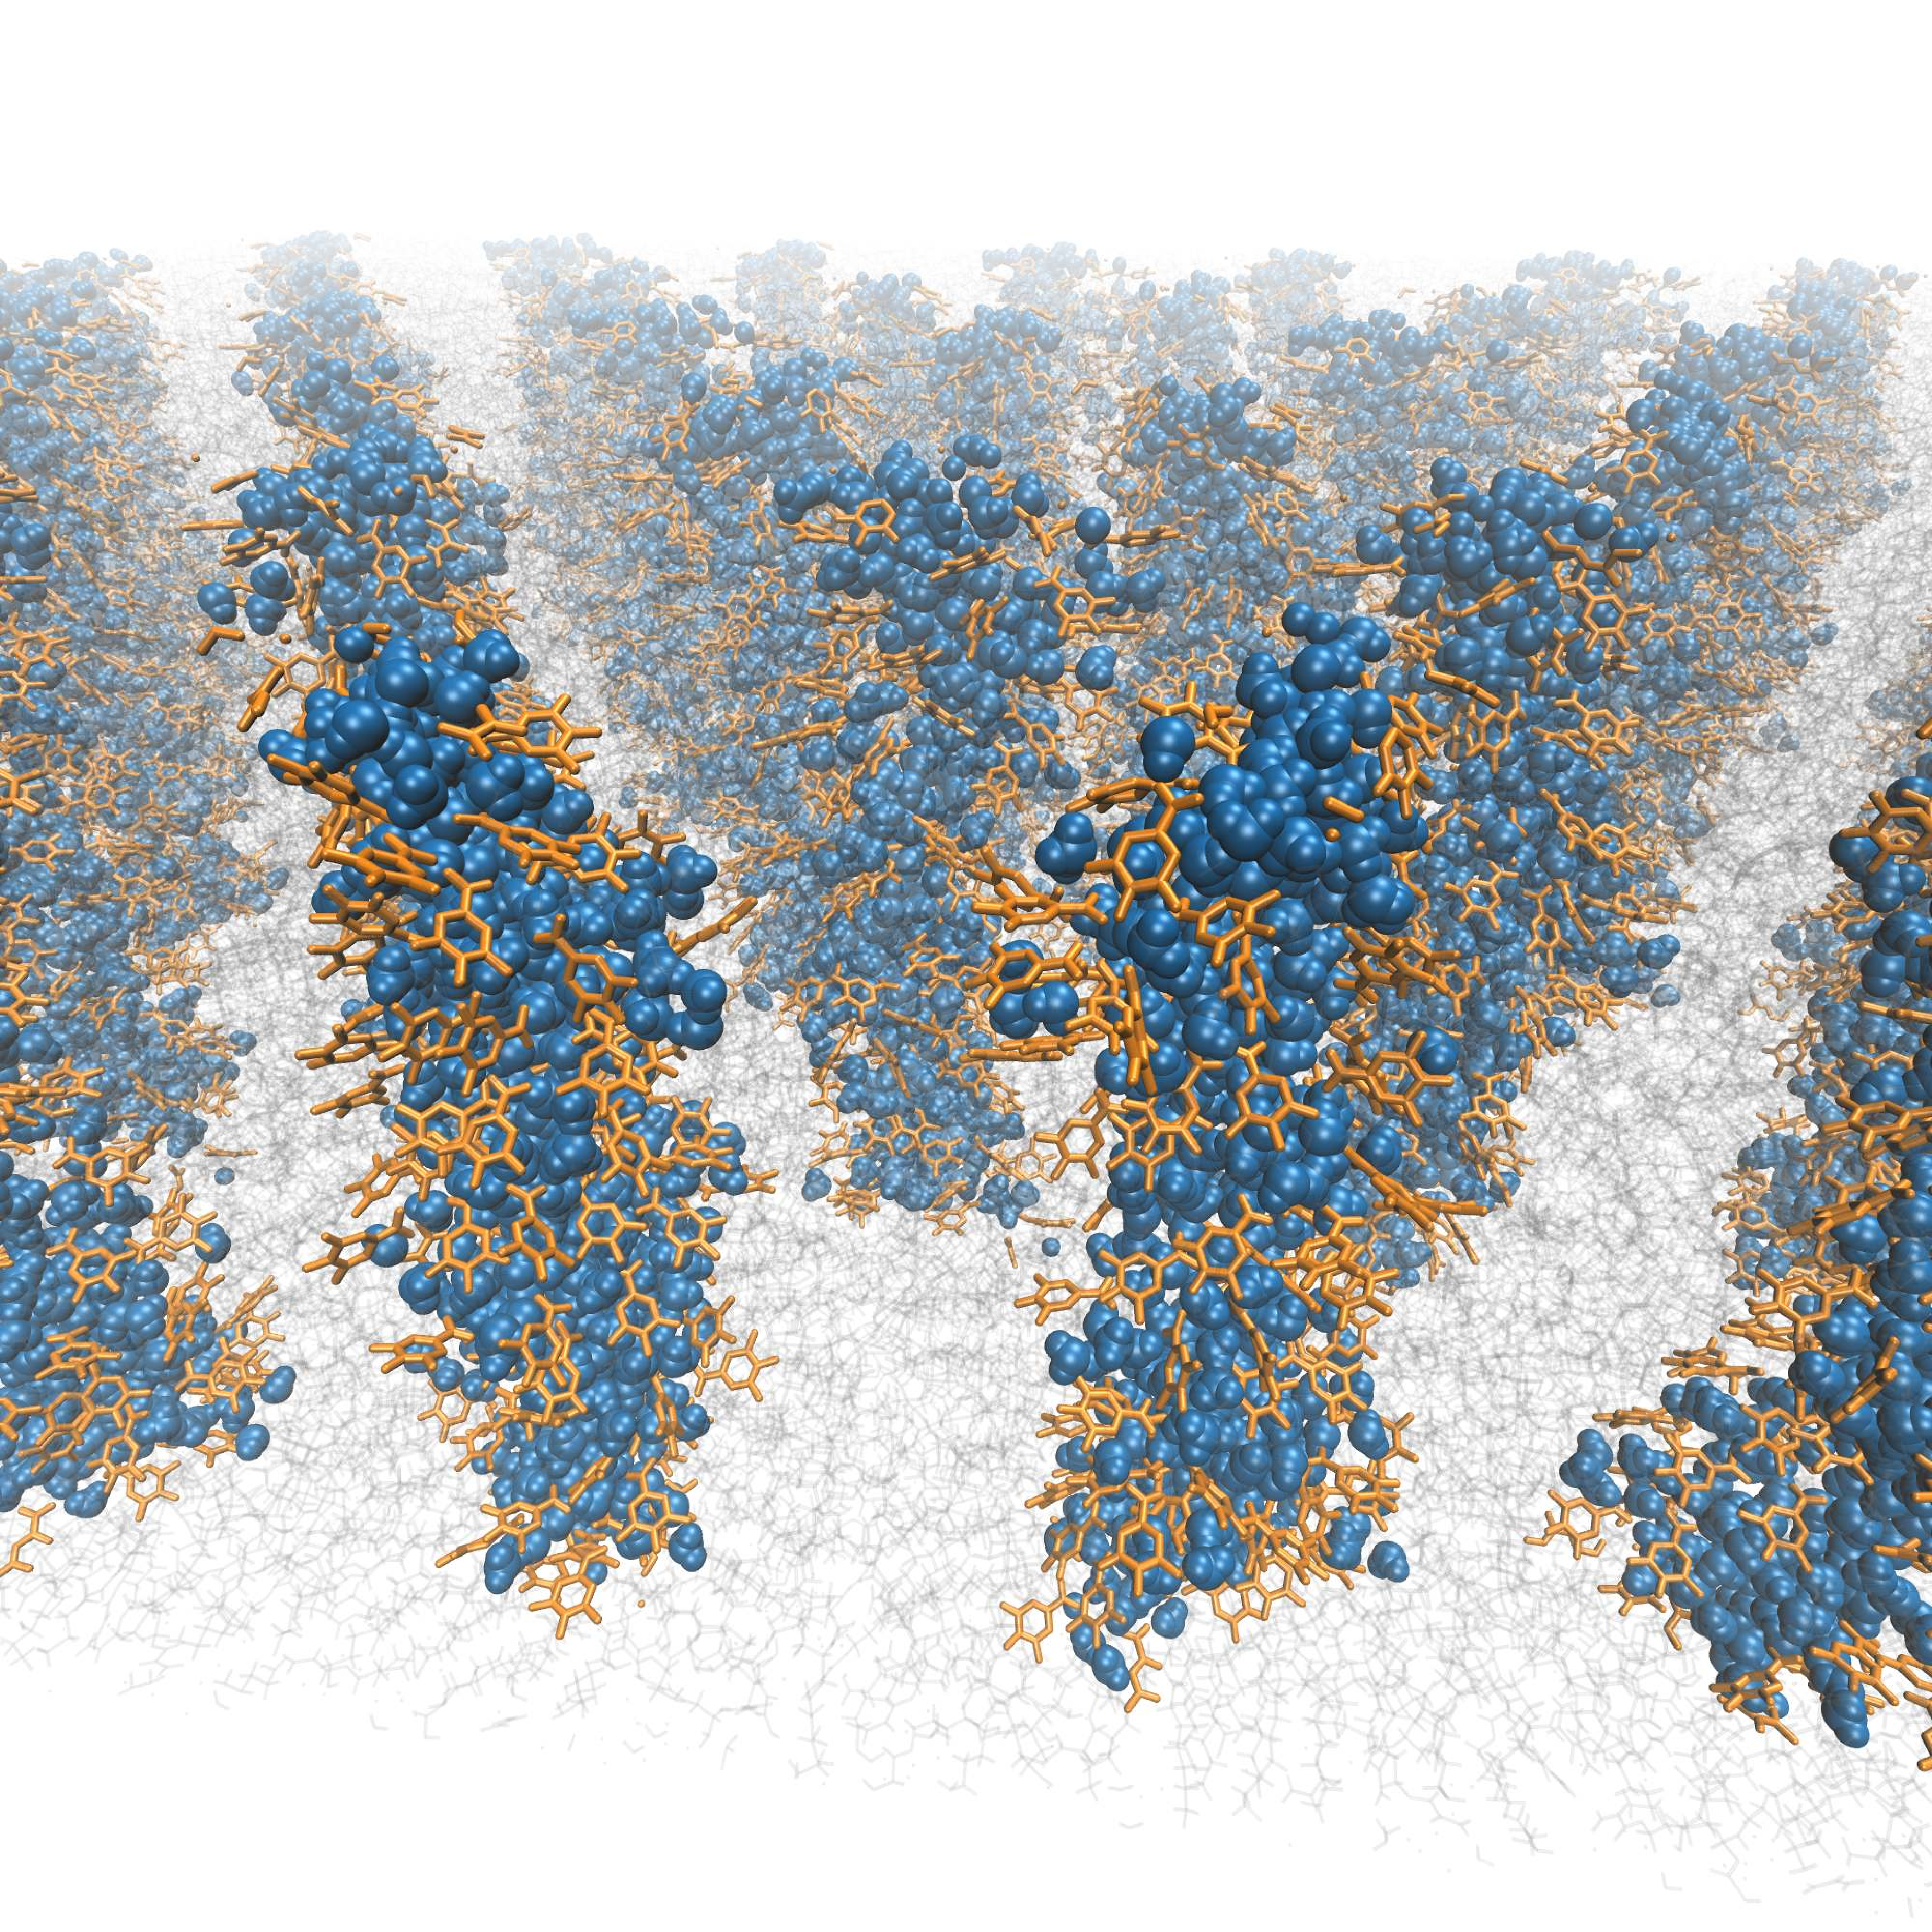
\includegraphics[width=\textwidth]{ortho_view.pdf}
  \caption{}
  \end{subfigure}
  \begin{subfigure}{0.45\textwidth}
  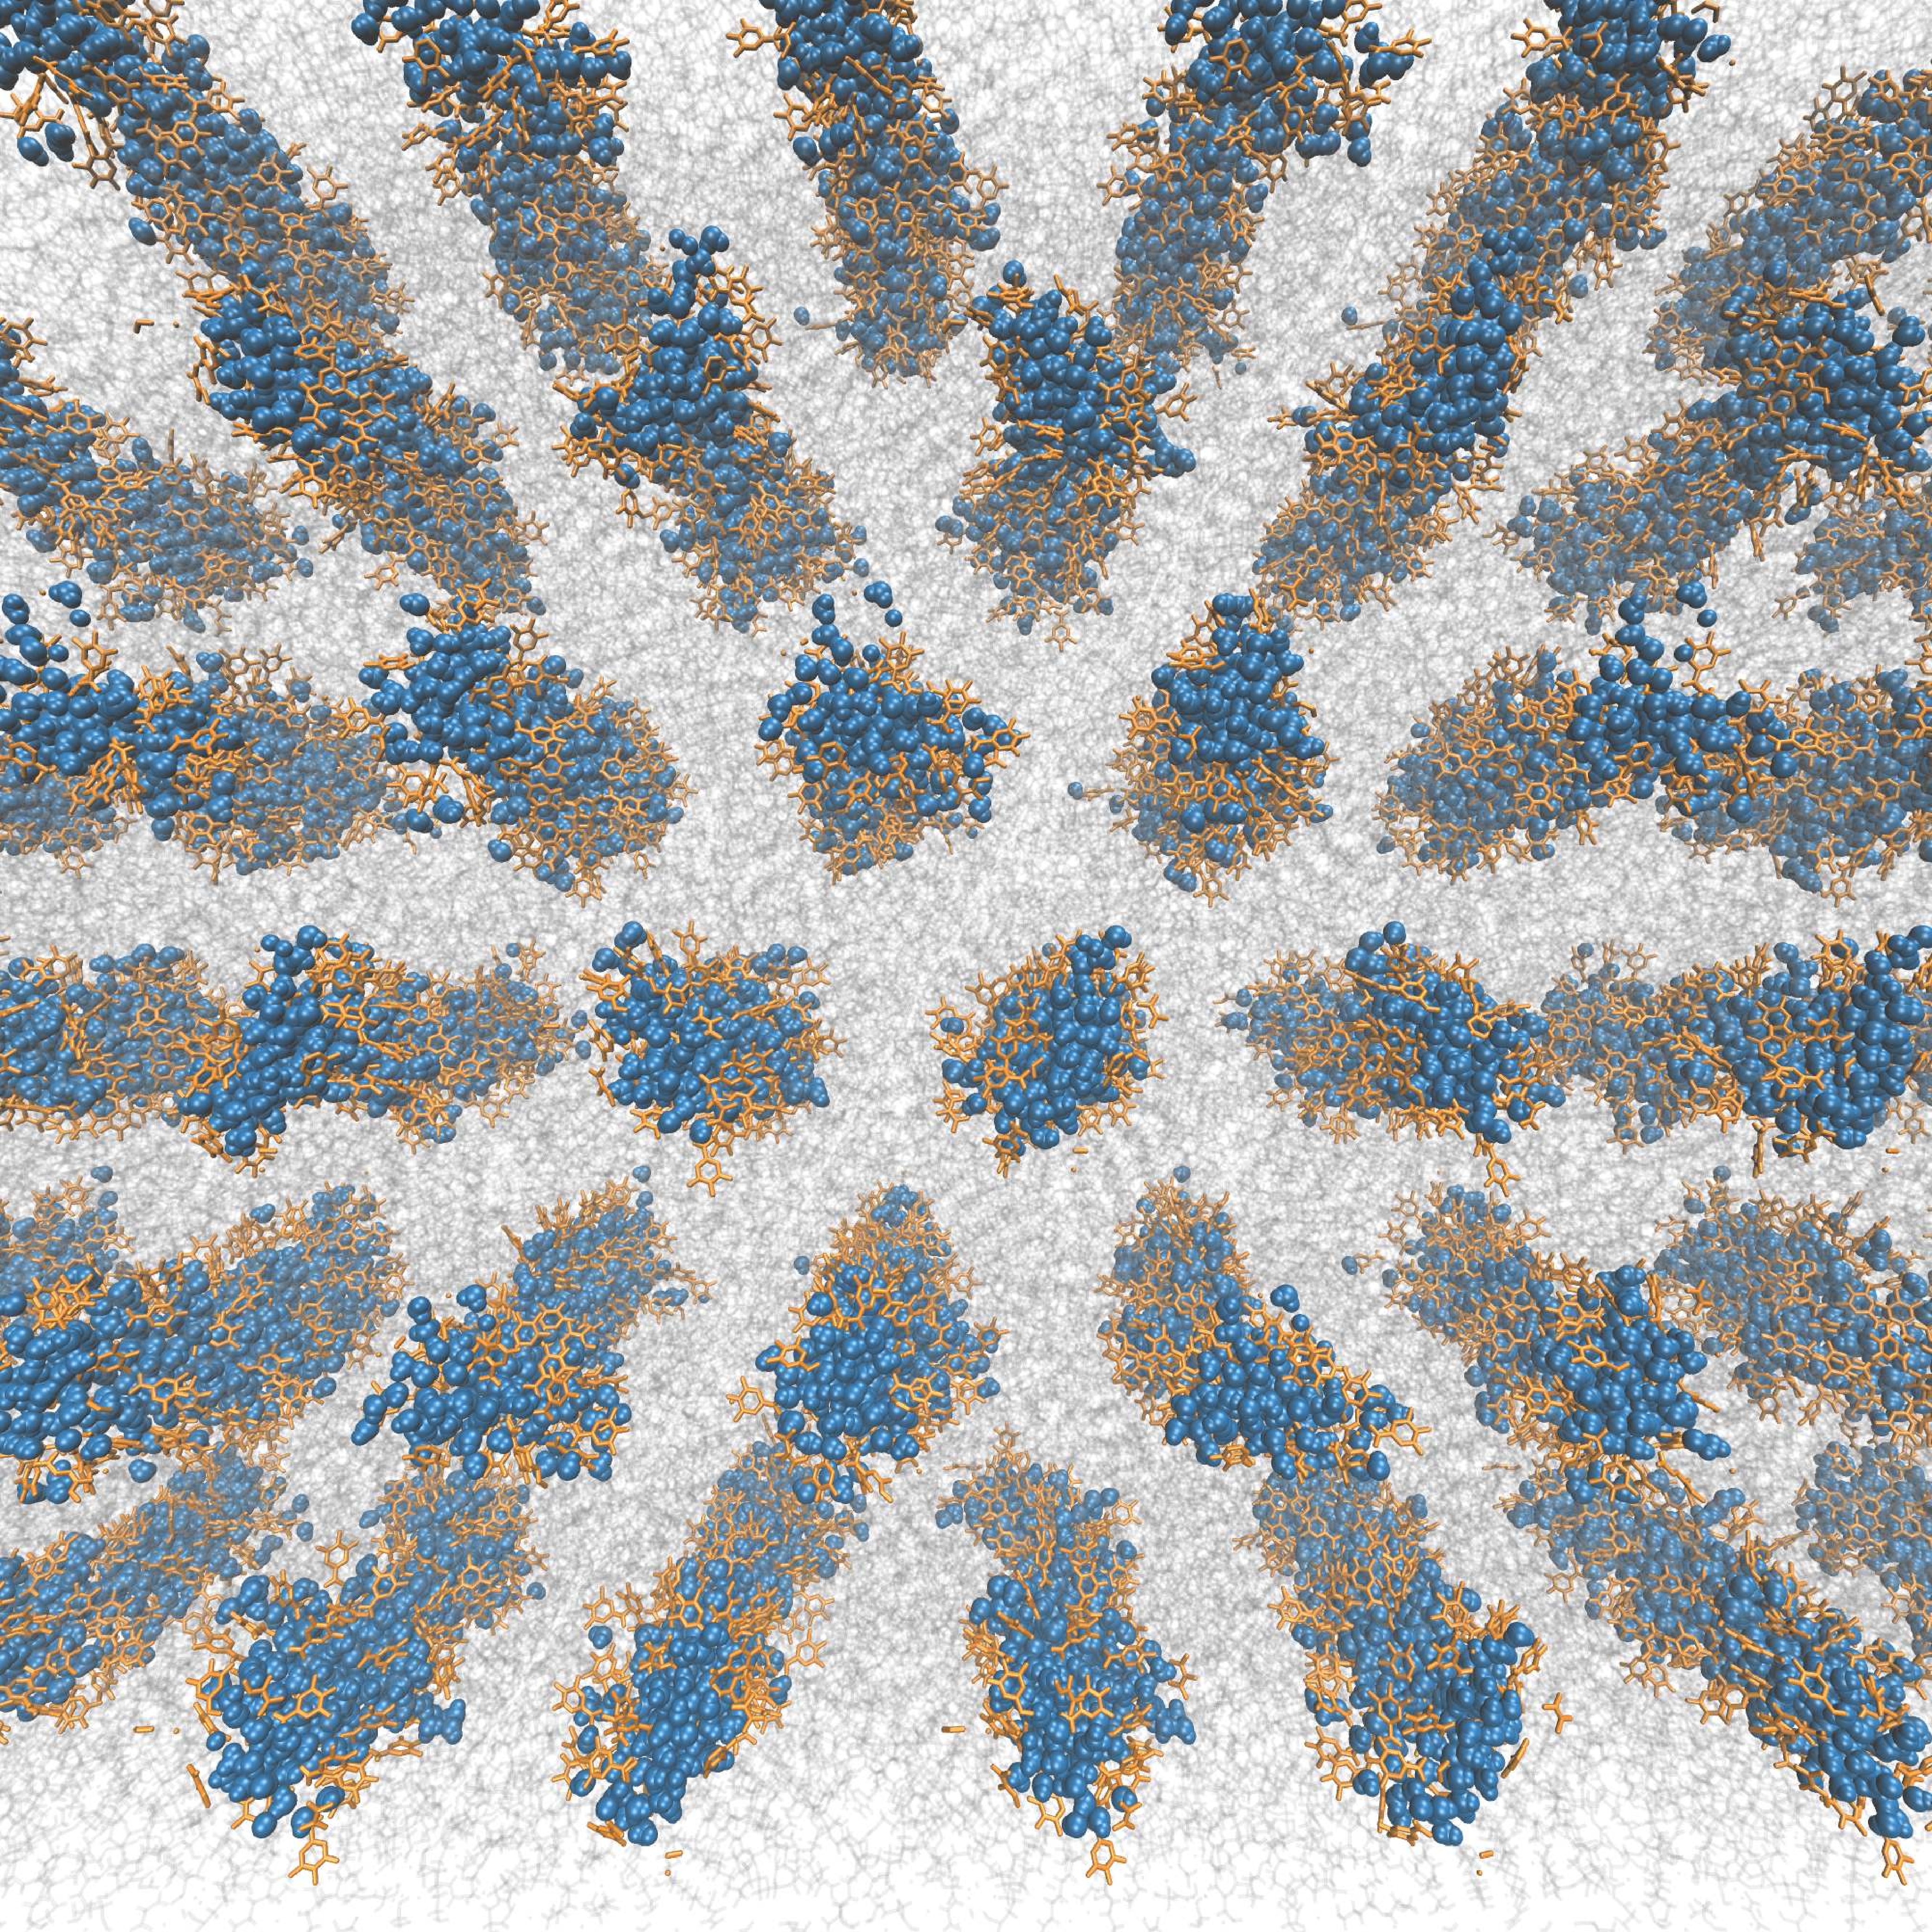
\includegraphics[width=\textwidth]{top_view.pdf}
  \caption{}
  \end{subfigure}
  %MRS3: include a bit more description in the caption of what the system: This is the figure that provides the orientation to the readers of what they will be thinking about for the rest of the paper.
  %BJC3: gave it another shot
  \caption{The H\textsubscript{II} phase formed by LLC monomers consists of pores
  that are approximately straight (a) and packed hexagonally (b). In both figures,
  water molecules that occupy the pores are colored blue, the hydrophilic head 
  groups of the LLC monomers are colored orange and all else is colored gray. 
  The chemical environment within the nanopores is largely determined by the functionality
  of the head groups. Additionally, there is not a well-defined transition
  point from the aqueous pore region to the alkane-dense, hydrophobic tail region,
  generating further complexity.
  }\label{fig:membrane_rendering}
  \end{figure}

  \begin{table}[h!]
  \centering
  \begin{tabular}{ |m{3.5cm}m{1.4cm}m{2cm}|m{3.8cm}m{1.4cm}m{2cm}| }
    \hline
    \multicolumn{2}{|c}{Solute Name~~~~~~~~~Abbreviation} & Structure &\multicolumn{2}{c}{Solute Name~~~~~~~~~Abbreviation} & Structure \\
    \hline
	\color{blue}{\textbf{methanol}} & \color{blue}{\textbf{MeOH}} &     
    \begin{minipage}{.1\textwidth}
    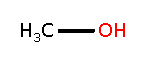
\includegraphics[width=\linewidth]{structures/MET.pdf}
    \end{minipage} &

    \color{green!40!olive}{\textbf{urea}} & \color{green!40!olive}{\textbf{URE}} &     
    \begin{minipage}{.1\textwidth}
    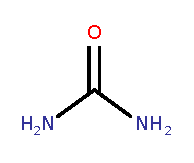
\includegraphics[width=\linewidth]{structures/URE.pdf}
    \end{minipage} \\
    
   	\color{blue}{\textbf{ethanol}} & \color{blue}{\textbf{EtOH}} &     
    \begin{minipage}{.1\textwidth}
    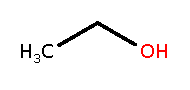
\includegraphics[width=\linewidth]{structures/ETH.pdf}
    \end{minipage} &
    
    \color{green!40!olive}{\textbf{acetamide}} & \color{green!40!olive}{\textbf{AcN}} &     
    \begin{minipage}{.1\textwidth}
    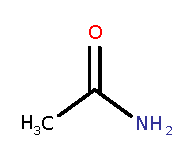
\includegraphics[width=\linewidth]{structures/ACN.pdf}
    \end{minipage} \\
    
  	\color{blue}{\textbf{propanol}} & \color{blue}{\textbf{PrOH}} &     
    \begin{minipage}{.1\textwidth}
    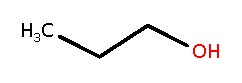
\includegraphics[width=\linewidth]{structures/PR.pdf}
    \end{minipage} &
    
    \color{green!40!olive}{\textbf{acetone}} & \color{green!40!olive}{\textbf{ACE}} &     
    \begin{minipage}{.1\textwidth}
    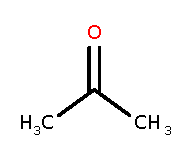
\includegraphics[width=\linewidth]{structures/ATO.pdf}
    \end{minipage} \\
    
    \color{blue}{\textbf{butanol}} & \color{blue}{\textbf{BtOH}} &     
    \begin{minipage}{.1\textwidth}
    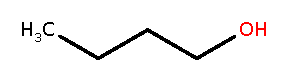
\includegraphics[width=\linewidth]{structures/BUT.pdf}
    \end{minipage} &
    
    \color{orange}{\textbf{mercaptoethanol}} & \color{orange}{\textbf{ME}} &     
    \begin{minipage}{.1\textwidth}
    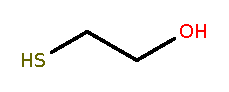
\includegraphics[width=\linewidth]{structures/SOH.pdf}
    \end{minipage} \\
    
    \color{red}{\textbf{ethylene glycol}} & \color{red}{\textbf{EG}} &     
    \begin{minipage}{.1\textwidth}
    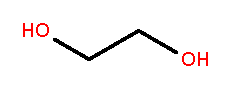
\includegraphics[width=\linewidth]{structures/GCL.pdf}
    \end{minipage} &

    \color{orange}{\textbf{dimethyl sulfoxide}} & \color{orange}{\textbf{DMSO}} &     
    \begin{minipage}{.1\textwidth}
    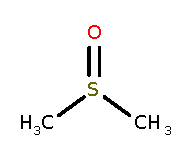
\includegraphics[width=\linewidth]{structures/DMS.pdf}
    \end{minipage} \\
    
    \color{red}{\textbf{propylene glycol}} & \color{red}{\textbf{PG}} &     
    \begin{minipage}{.1\textwidth}
    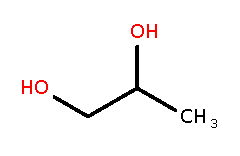
\includegraphics[width=\linewidth]{structures/PG.pdf}
    \end{minipage} &
    
    \color{orange}{\textbf{2,3-dimercapto-1-propanol}} & \color{orange}{\textbf{DMP}} &     
    \begin{minipage}{.1\textwidth}
    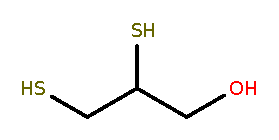
\includegraphics[width=\linewidth]{structures/DMP.pdf}
    \end{minipage} \\
    
    \color{red}{\textbf{glycerol}} & \color{red}{\textbf{GLY}} &     
    \begin{minipage}{.1\textwidth}
    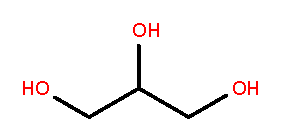
\includegraphics[width=\linewidth]{structures/GLY.pdf}
    \end{minipage} &

    \color{amber}{\textbf{tetrahydrofuran}} & \color{amber}{\textbf{THF}} &     
    \begin{minipage}{.1\textwidth}
    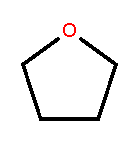
\includegraphics[width=\linewidth]{structures/THF.pdf}
    \end{minipage} \\
    
    \color{red}{\textbf{tetrose}} & \color{red}{\textbf{TET}} &     
    \begin{minipage}{.1\textwidth}
    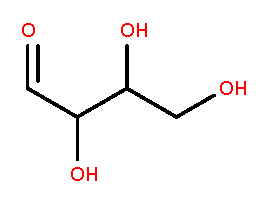
\includegraphics[width=\linewidth]{structures/TET.pdf}
    \end{minipage} &
    
    \color{amber}{\textbf{dimethylformamide}} & \color{amber}{\textbf{DMF}} &     
    \begin{minipage}{.1\textwidth}
    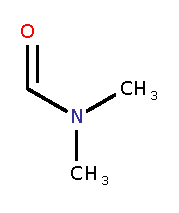
\includegraphics[width=\linewidth]{structures/DMF.pdf}
    \end{minipage} \\
    
    \color{red}{\textbf{ribose}} & \color{red}{\textbf{RIB}} &     
    \begin{minipage}{.1\textwidth}
    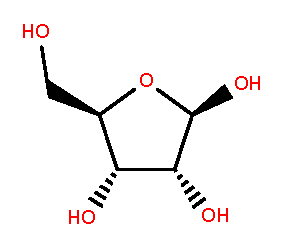
\includegraphics[width=\linewidth]{structures/RIB.pdf}
    \end{minipage} &

    \color{amber}{\textbf{propylene carbonate}} & \color{amber}{\textbf{PC}} &     
    \begin{minipage}{.1\textwidth}
    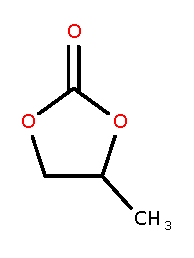
\includegraphics[width=\linewidth]{structures/PCB.pdf}
    \end{minipage} \\
    
    \color{green!40!olive}{\textbf{acetic acid}} & \color{green!40!olive}{\textbf{AcOH}} &     
    \begin{minipage}{.1\textwidth}
    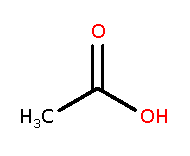
\includegraphics[width=\linewidth]{structures/ACH.pdf}
    \end{minipage} &

    \color{amber}{\textbf{ethyl acetate}} & \color{amber}{\textbf{EAC}} &     
    \begin{minipage}{.1\textwidth}
    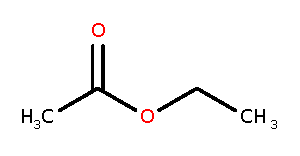
\includegraphics[width=\linewidth]{structures/EAC.pdf}
    \end{minipage} \\
  
    \hline
  \end{tabular}
  \caption{Names of solutes along with their molecular structures and the
  abbreviations which we use in this paper. Colors correspond to solute groupings
  and are used in many plots. 
%  Blue corresponds to simple alcohols, red to 
%  diols, triols and sugars, green to ketone-like solutes, orange to sulfur-containing
%  solutes and yellow to solutes that can only accept hydrogen bonds but not donate.
  }\label{table:abbreviations}
  \end{table}

  %MRS2: generally, use present tense for what is being done in the paper, not future tense; 
  %the paper is completely written, later sections are not being written in the future. 
  %MRS2: descriptions of experiments can be in the past.   
  %MRS2: look over this section at the end of the intro again for clarity - some paragraphs are too short (ideas introduced and brushed past quickly) sometimes without strong theses.
  %BJC3: I think these make more sense now. 
  
  We first address the structure of the membrane nanopores. Previously, we
  studied dry membrane systems and some systems with low water content. We showed
  that those systems have rather crowded pores with high concentrations of monomer
  head groups, sodium ions and water, where applicable. Here we build systems with
  appreciable amounts of water, 5 and 10\% by weight, and analyze how the radial
  density of monomer components and water change compared to our previous results.

%  We then present our efforts to understand how water partitions within the pores.  
  We then use the transport rates of water in and out of the pores in order to
  to justify our study of solute transport restricted to the pore region. From a 
  macroscopic perspective, it might make sense to hypothesize that water spends its time 
  exclusively in the tube-like hydrophilic pore region. Our previous work showed
  that there is a gradual compositional transition from the hydrophilic to the
  hydrophobic region which means that solutes may not necessarily stay confined
  to the centers of the pores or even within the pore region. We show that, in 
  our most viable system, water moves fastest within the pores suggesting that 
  the 
  %MR3: added to be more specific - we do look at it getting into the head groups a little.
  area in and around the central
  pores should be the focus of our mechanistic studies.
  
  %MRS2: ``this information'' is ambiguous. Which information? Also, I'm not sure the paragraph above is enough to 
  %demonstrate why we can/should neglect the tails.
%  We use this information in order to justify our restriction
%  of solute transport studies to just the pore region.
  
%  We then study the gradient in composition of solutes and 
%  water and any resultant influence it might have on mechanistic properties.

  In the remainder of the paper, we describe and quantify three trapping 
  mechanisms which give rise to subdiffusive solute transport behavior. 
  We describe the differences in solute motion, specifically their mean
  squared displacement (MSD), in conjunction with each solute's size and 
  chemical functionality. We show how distinct interactions with various
  monomer components as well as membrane water content hinders the motion 
  of solutes. We discuss how the interactions between specific solutes and
  the membrane depend on the solute's chemical functionality.

  There are also several questions beyond the scope of this study.
  First, we will not study the concentration dependence of the observed transport
  rates. Although the average MSD might change with concentration, we are 
  focused on the underlying solute-membrane interactions that lead to the 
  observed transport mechanisms which we conjecture will remain roughly
  the same regardless of concentration. Second, we will not study the chemical potential
  of solutes in the pores, which could give us a better understanding of 
  equilibrium solute partitioning. However, this information is likely
  not needed to understand the principal mechanistic details in various membrane
  regions. This work instead represents a starting point for observing the 
  types of interactions that occur between isolated solutes and the membrane.

  \section{Methods}
  
  Python scripts used to set up systems and conduct post-simulation trajectory 
  analysis (as described below and in the supporting information) are available 
  online at \texttt{https://github.com/shirtsgroup/LLC\_Membranes}. The 
  appropriate scripts to use for the subsequent calculations are summarized in 
  Table~\ref{S-table:python_scripts} of the Supporting Information. We ran all 
  MD simulations and energy minimizations using GROMACS 2018.3.~\cite{bekker_gromacs:_1993,berendsen_gromacs:_1995,van_der_spoel_gromacs:_2005,hess_gromacs_2008} 
  
  \subsection{Solute Parameterization}\label{method:parameterization}
  
  We parameterized the interaction potential for the monomer and solutes using 
  the Generalized AMBER Force Field (GAFF)~\cite{wang_development_2004} with the
  Antechamber package \cite{wang_automatic_2006} shipped with AmberTools16~\cite{case_ambertools16_2016}.
  We use GAFF as it has been used extensively for use with organic molecules.
  We assigned atomic charges using the am1bccsym method of \texttt{molcharge} included
  with QUACPAC from OpenEye Scientific Software.
  
  \subsection{System Setup}\label{method:system_setup}

  Stable H\textsubscript{II} phases, assembled with Na-GA3C11, can be formed
  using a broad range of water concentrations. In the literature, the system 
  studied in this work is typically synthesized with close to 10 wt\% water.
  \cite{smith_ordered_1997, zhou_new_2007} However, Resel et al. noted that the
  system is likely fully hydrated with less than 7 wt\% water.~\cite{resel_h2-phase_2000}
  Excess water fills space between hexagonal mesophases. We decided to test 
  systems with two different water contents: 5 and 10 wt\%.

  We observed that some water partitions into the distal tail region of our system and therefore
  built our initial configurations with water in both regions, close to the expected
  equilibrium partition (see Section~\ref{S-section:water_content_equil} of the Supporting
  Information). We define the distal tail region to be ca. 1.5 nm from the pore
  center based on the minimum in the radial distribution of water
  (see Section~\ref{method:rdfs}). The amount of water present in the distal tail region
  may or may not be experimentally consistent but it is necessary for our results to be 
  thermodynamically consistent; otherwise, water would slowly leak from the pore into the
  tail region over several hundred nanoseconds. We iteratively adjusted the pore radius in our systems
  until the appropriate amount of water fit in the pores after running the GROMACS command
  \texttt{gmx solvate}. We placed water molecules in the distal tail region one at a time
  in random locations with a short energy minimization between each insertion. When 
  studying transport of water in the pores, we limited the calculations to water molecules
  that spent greater than 95\% of their time outside of the distal tail region. We 
  justify this decision with better context in Section~\ref{section:transport_water_sodium}.
  %MRS2: seems like here is where we need to provide the justification for this decision, since the decision is described here (or, explain how we will justify it later)
  %BJC3: added reference to later section. 
  %MRS3: We probably need to mention the amount of water there is; 40% is in the tail.  We should probably discuss density; that because of the larger tail volume, the density is about 1/X in the distal region than in the pore.

  We equilibrated an initial solvated configuration before adding solutes. First, we 
  equilibrated the initial configuration using the `wet' equilibration procedure 
  described in our previous work. Then we cross-linked the equilibrated solvated 
  configuration using the cross-linking procedure also described in our previous 
  work.~\cite{coscia_understanding_2019}

  To study a given solute, we added 6 solute molecules, equally spaced in $z$, to the
  center of each pore of the equilibrated cross-linked configuration, for a total of 24
  solute molecules. We chose 6 solutes per pore to provide a balance of a useful amount of 
  data for generating statistics and a low degree of interaction between solutes (see 
  Section~\ref{S-section:solute_interaction} of the Supporting Information). At each
  insertion point we placed a randomly oriented solute molecule then ran a short 
  energy minimization. We allowed the solutes to equilibrate for 5 ns using Berendsen
  pressure control then collected transport data over the course of 1 $\mu$s MD simulations
  with pressure controlled by the Parrinello-Rahman barostat.

  %MRS2: could potentially make these sections bulleted list, rather than full subsections.
  \subsection{Mean Squared Displacement}\label{method:MSD}

  We measured the time-averaged $z$-direction (parallel to the pores) mean squared
  displacement (MSD) of the centers of mass (COM) of each solute over the course of 
  1 $\mu$s MD simulations using 
  Equation~\ref{eqn:tamsd}:
  \begin{equation}
	\overline{z^2(\tau)} = \dfrac{1}{T - \tau}\int_{0}^{T - \tau} (z(t + \tau) - z(t))^2 dt
	\label{eqn:tamsd}
  \end{equation}
  where $\tau$ is the time lag and T is the length of the trajectory~\cite{meroz_toolbox_2015}. 
  The MSD, in standard treatments, grows according to Equation~\ref{eqn:msd_form}:
  \begin{equation} 
	\langle z^2(t) \rangle = K_{\alpha}t^\alpha
	\label{eqn:msd_form}
  \end{equation} 
  where $\alpha$ is the anomalous exponent and $K_\alpha$ is the generalized diffusion 
  coefficient. A value of $\alpha < 1$ indicates a subdiffusive process, while a value 
  of $\alpha = 1$ and $\alpha > 1$ is characteristic of Brownian and superdiffusive
  motion respectively.
    % MRS1: time vs. ensemble MSD better in follow-up paper.
    % BJC2: I think it makes sense to mention, otherwise it looks like we don't 
    % fully understand the theory since I talk about subdiffusion in terms of 
    % alpha which is always calculated based on ensemble MSD unless we know for sure that
    % the system is ergodic (which it isn't the case for CTRW)
  In practice, $\alpha$ corresponds to the growth of the \textit{ensemble} MSD given
  by Equation~\ref{eqn:ensemble_msd}~\cite{meroz_toolbox_2015}:
  \begin{equation}
	\langle z^2(t) \rangle = \langle z(t) - z(0) \rangle
	\label{eqn:ensemble_msd}
  \end{equation}
  Since the ensemble MSD is calculated with respect to a reference position, it carries
  some dependence on its starting point. The time-averaged MSD averages over all possible
  time lags of a given length, effectively eliminating any initial configuration 
  dependence and generating	an increased number of observations. For ergodic systems, 
  both types of MSDs will be equal. Since we have a small number of solutes with which to
  generate statistics and because we are not calculating values of $\alpha$ for this 
  particular study,	we will only use the time-averaged MSD.
  
  % BJC: haven't talked about hopping mechanism at this point, but need to justify why
  % I used total MSD rather than fitting some function to it
  We fixed the length of each simulated trajectory so that we could compare the total
  MSD between different solutes without the influence of the ageing phenomenon.
  In systems such as ours where solutes show hopping behavior between long periods 
  of immobility, ageing is defined by the tendency of the average slope of an MSD 
  curve to decrease as the length of trajectories are increased~\cite{metzler_anomalous_2014}.
  Since the maximum measured dwell time can be no longer than the total length of a simulated
  trajectory, longer dwell times are incorporated into the calculation as measurement
  time or trajectory length is increased, lowering the average MSD. Because the solute 
  MSDs are non-linear and because of the ageing phenomenon, we did not attempt to calculate
  a diffusion constant as one might for a Brownian particle with a linear MSD. Instead,
  the reported MSD values represent the average MSD for a given	solute after a 400
  ns time lag. Our results are shown to be insensitive to our choice of time lag in 
  Section~\ref{S-section:lag_sensitivity} of the Supporting Information.
  
  The $z$-direction MSD of water in the 10 wt\% system \textit{is} linear to within 
  statistical precision. Therefore, for the purpose of comparison, we calculated its
  %BJC3: linear within statistical precision --> appears linear? I didn't do any rigorous tests for linearity
  diffusion constant by fitting a line to the linear region of the MSD curve.~\cite{maginn_best_2018}. The diffusion constant
  is then equal to $m/2$ where $m$ is the slope of the linear fit. The slope is divided
  by 2 (rather than 6) because we only measured particle displacement in one dimension.

  \subsection{Molecular Size Determination}\label{method:molecular_size}
  
  In order to determine an effective radius for each solute, we divided in 
  half the maximum pairwise distance between atoms of each solute over the course of
  a 2.5 ns simulation of solutes dissolved in a cubic box of water. Each box 
  consisted of about 2100 water molecules and 6 solutes. Although there exist
  more involved methods for determining the hydrodynamic radius~\cite{schultz_determination_1961},
  we chose to use a simpler and more intuitive metric since we are only interested
  in observing trends in the solute MSD as a function
  of solute size.
  
  \subsection{The Stokes-Einstein Relationship}\label{method:stokes}
  
  The Stokes-Einstein relationship expresses the diffusion coefficient of 
  a hard spherical particle as a function that is inversely related to the
  particle's radius:
  \begin{equation}
  D = \dfrac{k_bT}{6\pi\eta fr}
  \label{eqn:stokes-einstein}
  \end{equation}
  where $k_b$ and $T$ are the Boltzmann	constant and the system temperature
  respectively and $\eta$ is the system's viscosity. Here we have also 
  included the microfriction correction factor, $f$, introduced by 
  Gierer and Wirtz~\cite{gierer_molekulare_1953,chen_diffusion_1984} for when
  solute size becomes on the order of solvent size since the solute can no 
  longer be treated as a non-interacting hard sphere. $f$ is defined in terms
  of the ratio of $r_1$ and $r_2$, the radii of the solute and solvent molecules
  respectively:
  \begin{equation}
  f = \left(1.5\dfrac{r_2}{r_1} + \dfrac{1}{1 + \dfrac{r_2}{r_1}}\right)^{-1}
  %f = \left(1.5(r_2/r_1) + \dfrac{1}{1 + (r_2/r_1)}\right)^{-1}
  \label{eqn:correction_factor}
  \end{equation}
  For consistency with the presentation of our results, rather than calculate 
  trends in $D$, we will calculate trends in trends in solute MSDs. For Brownian
  particles, $D$ is proportional to the MSD divided by time, $t$. Therefore, 
  we analyze qualitative trends in solute MSDs according to:
  \begin{equation}
  MSD = \dfrac{k_bTt}{6\pi\eta fr}
  \label{eqn:msd-stokes-einstein}
  \end{equation}
  We hold $t$ constant in our simulations in order to make side-by-side comparisons. 

  %MRS4: a bit strange to say you are using Stokes-einstein, but only analyzing MSD's (when MSD's don't appear in that equation)? It could be clarified a bit more.
%  However, this assumes linear behavior
%  of the MSD, which we will show is not that case. Our main usage of the 
%  Stokes-Einstein relationship is to show that solutes in our system do not 
%  behave as it predicts.
  % Possible comps question: Stokes law restricted to Re < 0.1, but we have no flow so Re ~ 0.
  
  Since we will be using Equation~\ref{eqn:msd-stokes-einstein} for primarily qualitative observations, 
  we made a number of simplifying assumptions so that it could easily be used for 
  comparison between systems. First, we assume that all systems' viscosities
  are equal since we only make minor changes to the membrane's composition and
  accurately assessing the viscosity in a complex and inhomogeneous system such 
  as ours is a challenge by itself. Second, we assume all particles are approximately
  spherical, neglecting the effect of solute shape on mobility. Chan et al. 
  showed that the difference in diffusion constants of differently shaped 
  particles, with constant molecular volume, did not differ by more than 25\%
  with most deviating by less than 10\%.~\cite{chan_effects_2015}. 
  Third, we assume that the ratio of solute and solvent radii as calculated using the
  methodology of Section~\ref{method:molecular_size}, is equivalent to the the 
  ratio of hydrodynamic radii. For similarly shaped molecules, it has been shown that
  one can relate the hydrodynamic radius and radius of gyration (R\textsubscript{g})
  using a constant scaling factor. \cite{lee_molecular_2008,he_novel_2003,li_critical_2009}.
  % BJC: could just calculate Rg instead of end-to-end
  Assuming that our end-to-end distance reasonably approximates R\textsubscript{g} 
  for our small, relatively inflexible molecules, we believe this assumption is 
  justified for qualitative demonstrations relevant to this study. 
  
  %BJC: another option is to fit to water which IS Brownian in the 10 wt% system.
  In order to make qualitative comparisons, we fit Equation~\ref{eqn:msd-stokes-einstein}
  so that it passed through the highest solute MSD. We assumed that the solute
  with the highest MSD exhibited the closest to Brownian behavior and therefore could set
  a rough boundary between subdiffusive, Brownian and superdiffusive MSDs. As a lower
  bound to our appoximation, we also plotted the uncorrected version of 
  Equation~\ref{eqn:stokes-einstein} ($f$=1), requiring it to converge to the same 
  value as the corrected curve for large radii. 
  % BJC: Set really high intersection value. Converges quickly (i.e. critical radius
  % (the radius where curves intersect) of 2.5 nm looks almost the same as critical
  % radius of 100 nm. I don't think this necessarily needs to be proved anywhere

%  at the critical particle radius 
%  where the uncorrected Stokes-Einstein begins to break down. An exact critical
%  radius is not well-defined, but based on the observations of others, we will
%  approximate that radius as 2.5 nm\cite{li_critical_2009,polson_some_1950}. The 
%  sensitivity of the uncorrected curve to this intersection radius is shown to 
%  be small and is graphically illustrated in Section-TBD of the Supporting Information.
  
%  It is well-known that equation~\ref{eqn:stokes-einstein} breaks down Gierer and Wirtz introduced a microfriction
%  correction factor in order to address this issue. 
%  They proposed that 
%  \begin{equation}
%  D = \dfrac{k_bT}{6\pi\eta fr}
%  \end{equation}
%  where 

  \subsection{Hop Detection}\label{method:hop_detection}
  
  In order to measure the length of hops, we first needed to detect
  when they occurred. We used an off-line change point detection 
  algorithm, implemented in the python package \texttt{ruptures}
  \cite{truong_ruptures:_2018}, in order to determine at which 
  points hops occurred in the time series of each solutes' COM. We
  used the 3 dimensional COM positions of each solute, rather than
  just the $z$-direction, in order to detect lateral hops. However,
  hop lengths are reported as their displacement in the $z$-direction.
  We reported the standard error in the average hop lengths by 
  bootstrapping the empirical distribution of observed
  hop lengths.\cite{efron_introduction_1994}

  We determined the average frequency of hops by dividing the total number of 
  hops by the total length of the simulation. We used the frequency of
  hops per 1000 ns as the $\lambda$ parameter in a Poisson distribution.
  We calculated the 1$\sigma$ confidence intervals of the probability % BJC: not sure best way to write 1-sigma CI
  distribution of hops per 1000 ns based on the corresponding Poisson 
  cumulative distribution function and scaled them to a per--nanosecond basis. 
 
%  We used the normal 
%  approximation in order to estimate the 95 \% confidence interval
%  of these estimates:
%  \begin{equation}
%  95\%~CI = 1.96 \sqrt{\dfrac{\lambda}{n}}
%  \end{equation}
%  where $\lambda$ is the average frequency of hops and n is the total
%  observation time accumulated for all solutes.
  
  We differentiated between the length of hops inside and outside of the 
  pores. For 10 wt\% water systems, we consider a solute to be in the pore
  if it is within 0.75 nm of a pore center. This radial cut-off maximizes 
  the difference between average hop lengths in and out of the pore. 
  See Section~\ref{S-section:pore-region} of the Supporting
  Information for further details on this optimization.
  
  \subsection{Time Spent in Pore Region}
  
  Using the cut-off defined above, we calculated the fraction of time
  that a solute spends within the pore region. Since this is a process
  with two possible outcomes, we calculated the standard error ($SE$) of our
  calculations based on the binomial theorem: 
  \begin{equation}
  SE = \sqrt{\dfrac{p(1-p)}{n}}
  \end{equation}
  where $p$ is the probability that a solute is in the pore region and
  $n$ is the sample size. Here $n$ is the total number of transitions
  between each region. 
  
  \subsection{Identification and Analysis of Hydrogen Bonds}\label{method:hbonds}  % Could just make title 'Hydrogen Bonds'

  Based on the geometric criteria proposed by Luzar and Chandler 
  \cite{luzar_effect_1996}, we determined a hydrogen bond to exist if the
  distance between the donor, D, and acceptor, A, atoms is less than 
  3.5 \AA~and the angle formed by D--H$\cdot\cdot\cdot$A is less than 30\degree. Attempts
  to describe a hydrogen bond in the context of molecular simulations has
  yielded a number of definitions with no true consensus 
  \cite{prada-gracia_quest_2013} especially since the geometry of hydrogen
  bonds has some dependence on the system being studied. The definition of
  Luzar and Chandler is easily visualized for trajectories using the 
  \texttt{hbonds} representation of the Visual Molecular Dynamics (VMD) software 
  package which allows us to directly check the validity of identified hydrogen bonds.
  In Section~\ref{S-section:hbond_sensitivity} of the Supporting Information, we
  show that our conclusions are insensitive to this definition within a 
  reasonable range of distances and angles. 
  
  We determined the average percentage of solutes
  which actively participated in a hydrogen bond interaction with monomers 
  each frame. Unless noted otherwise, we only counted unique solute--monomer
  hydrogen bond interactions, meaning solutes that hydrogen bond more than 
  once simultaneously were classified as a single pairing event. We determined
  the standard error of this calculation by bootstrapping over each solute's 
  trajectory. For each bootstrap trial, we randomly chose 24 solutes with 
  replacement and calculated the average active solute--monomer hydrogen bonds per frame.

  \subsection{Coordination Number}\label{method:coordination}

  We quantified the coordination of solute constituent atoms with sodium ions.
  For each frame, we counted the number of coordinated molecules to a
  given solute atom based on a distance cut-off. Using four different methods,
  Rowley and Roux observed peaks in the radial distribution function for sodium
  coordinated with water at an O--Na distance of between 2.3 and 2.5 \AA.
  \cite{rowley_solvation_2012} We used 2.5 \AA~as the distance cut-off in our
  calculations. We found that this approach is more useful than calculating 
  the 3D spherical radial distribution function because it gives detailed 
  frame-by-frame information rather than an average. 
  
  Using our procedure, we found that sodium ions in a solution of TIP3P water
  coordinate with an average of 3.6 water molecules. We created a 4 x 4 x 4
  nm cubic box of water with the GROMACS tool, \texttt{gmx solvate}. We used
  \texttt{gmx genion} to replace water molecules with sodium and chloride 
  ions in order to create a 0.1 M NaCl solution. We let the system simulate
  for 5 ns and reported the average number of coordinated water molecules 
  per frame after discarding the first nanosecond of simulation.
  
  We determined the average percentage of solutes actively coordinated to
  a sodium ion each frame. Our calculation procedure is analogous to that for
  solute--monomer hydrogen bond interactions outlined in the previous section.
  
  \subsection{Association Lifetimes}\label{method:lifetimes}
  
  We quantified the length that two species stay associated via hydrogen
  bonding or coordination. For each unique pair, we measured the number of 
  consecutive frames in which they stayed associated. We considered pairs
  that disassociated for a single time step and reformed on the next time
  step as a single continuous association event. We compiled the length 
  of these events into a distribution of association lifetimes.
  %BJC: could justify why I didn't use autocorrelation functions
  
  % BJC: Clauset has an easily understood test for exponential versus power law. Would take
  % me maybe half a day to implement and generate results. Not sure if necessary though since
  % I'm just going to say that I don't know what distribution it is and we are going to
  % use a percentile.
  % MRS4: maybe while we are waiting for review.
  Hydrogen bond lifetimes appear to be distributed according to a power law or an
  exponential function (see Figure~\ref{S-fig:lifetime_distributions} of the 
  Supporting Information). A number of researchers provide evidence that supports a 
  power law distribution~\cite{starr_fast_1999,martiniano_insights_2013}. However, these
  studies were done on extremely short timescales relative to ours, outputting positions
  every time step. Voloshin et al. studied hydrogen bonding on multiple timescales and 
  observed exponential behavior on the longest timescales~\cite{voloshin_hydrogen_2009}. 
  Due to memory limitations, we could not collect data frequently enough to provide a
  sufficient answer to this question so when comparing solutes, we use the 95\textsuperscript{th} 
  percentile of hydrogen bond dwell times. This places emphasis on solutes with 
  long dwell times. We reported the standard error of this calculation by bootstrapping
  the distribution of dwell times.
  
  The distribution of sodium association lifetimes appear similar to
  hydrogen bond life time distributions. Therefore, we reported association
  lifetimes in the same manner as hydrogen bond lifetimes.
  
  \subsection{Radial Distribution Functions}\label{method:rdfs}

  We measured the average radial distance of each solute of interest 
  from the pore centers. We binned the radial distances and then 
  normalized by the volume of the annulus defined by the bin edges.
  We generated 1$\sigma$ confidence intervals by bootstrapping the 
  RDFs of each individual solute 200 times. For each solute, we obtained
  an RDF averaged over the entire simulation trajectory. We randomly 
  chose individual solute RDFs with replacement from the set of 24 and averaged 
  each set for each bootstrap trial in order to generate a distribution from 
  which to calculate uncertainties. 
  This approach assumes that solute positions are uncorrelated to
  other solutes which we believe is valid due to the low degree of 
  interaction between solutes described in Section~\ref{method:system_setup}.
  
  Although the pores are often described as straight, they have a
  small degree of tortuosity which disrupts the RDF calculation. We 
  tried to mitigate the effects of tortuosity by calculating the RDF
  with respect to splines that run through the pore centers. See
  Section~\ref{S-section:splines} of the Supporting Information for 
  a graphical illustration. Each spline consists of 10 points, equally
  spaced in the $z$-direction, whose ($x$, $y$) coordinates are defined
  based on the COM of all head groups closest, in $z$, to the
  given point. When calculating RDFs, the radial distance from the pore 
  center is based on the distance between the solute COM and
  the linearly interpolated ($x$, $y$) coordinates of the pore center 
  calculated based on the closest two spline points. Using the splines, 
  we calculated the tortuosity of the pores by calculating the ratio 
  $\dfrac{L}{Z}$ where $L$ is the length of the spline and $Z$ is the 
  length of the unit cell in the $z$-direction. The average tortuosity
  of each pore is 1.03 $\pm$ 0.01 and 1.07 $\pm$ 0.02 in the 5 and 10 wt\%
  water systems respectively.
  
  In all RDF plots, we include the average RDF of the head groups as a 
  reference. The head group RDF shown is the average of the head group
  RDFs for each solute system in the plot. We generated 1$\sigma$ 
  confidence intervals by bootstrapping the RDFs in the same way we did
  the solutes. We scaled the head group RDF so that it would be in frame
  next to solute RDFs.

%  of each individual
%  head group. For each head group, we obtained an RDF averaged over the
%  entire simulation trajectory. We randomly chose head group RDFs with replacement
%  and averaged them for each bootstrap trial. This approach assumes that
%  head group positions are uncorrelated.
   
  \section{Results and Discussion}
  
  \subsection{Structure of Membrane Constituents}\label{section:membrane_components} 
  
  Before beginning our analysis of solute transport behavior, it is important to
  elucidate the topology of the membrane pores in solvated systems.  
  
  In contrast to our previous work with a dry version of this membrane, the 
  region close to the pore center of the 5 and 10 wt\% water systems is 
  primarily filled with water and sodium ions. Figure~\ref{fig:component_densities}
  plots the RDF of each membrane constituent in the dry system as well as the
  5 and 10 wt\% water systems. In dry systems, the pore center is densely 
  filled with sodium ions and head groups. In hydrated systems, water occupies, 
  and is densest, at the center of each pore. The density of sodium ions is 
  somewhat uniform in the pore center of the 5 wt\% water system while it shows
  a maximum closer to the head groups in the 10 wt\% water system. The peak 
  density of sodium ions is not at the pore center in the 10 wt\% water system
  likely because they are associated with the monomer's carboxylate head groups.
  
  Pores in the 10 wt\% water system are wider and less crowded by monomers than
  those in the 5 wt\% water system. The peak head group density of 10 wt\% water
  systems is about 0.2 nm further from the pore center than the 5 wt\% water system. 
  Based on these observations, we expect solute transport to be fastest in the 
  10 wt\% water system.
  
  \begin{figure}[!htb]
  \centering
  \begin{subfigure}{0.45\textwidth}
  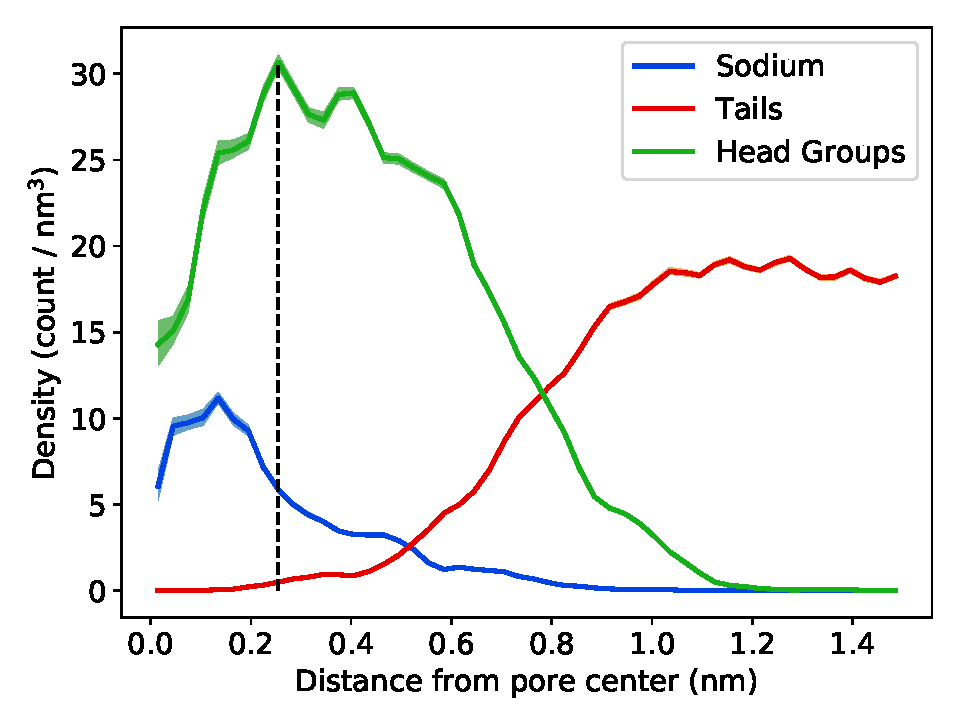
\includegraphics[width=\textwidth]{component_density_dry.pdf}  % running this out on bridges to make smoother
  %BJC: simulation is extended to smooth out these curves
  %BJC3: update: got slightly smoother
  \caption{Dry System}\label{fig:component_density_dry}
  \end{subfigure}
  \begin{subfigure}{0.45\textwidth}
  \vspace{-0.5cm}
  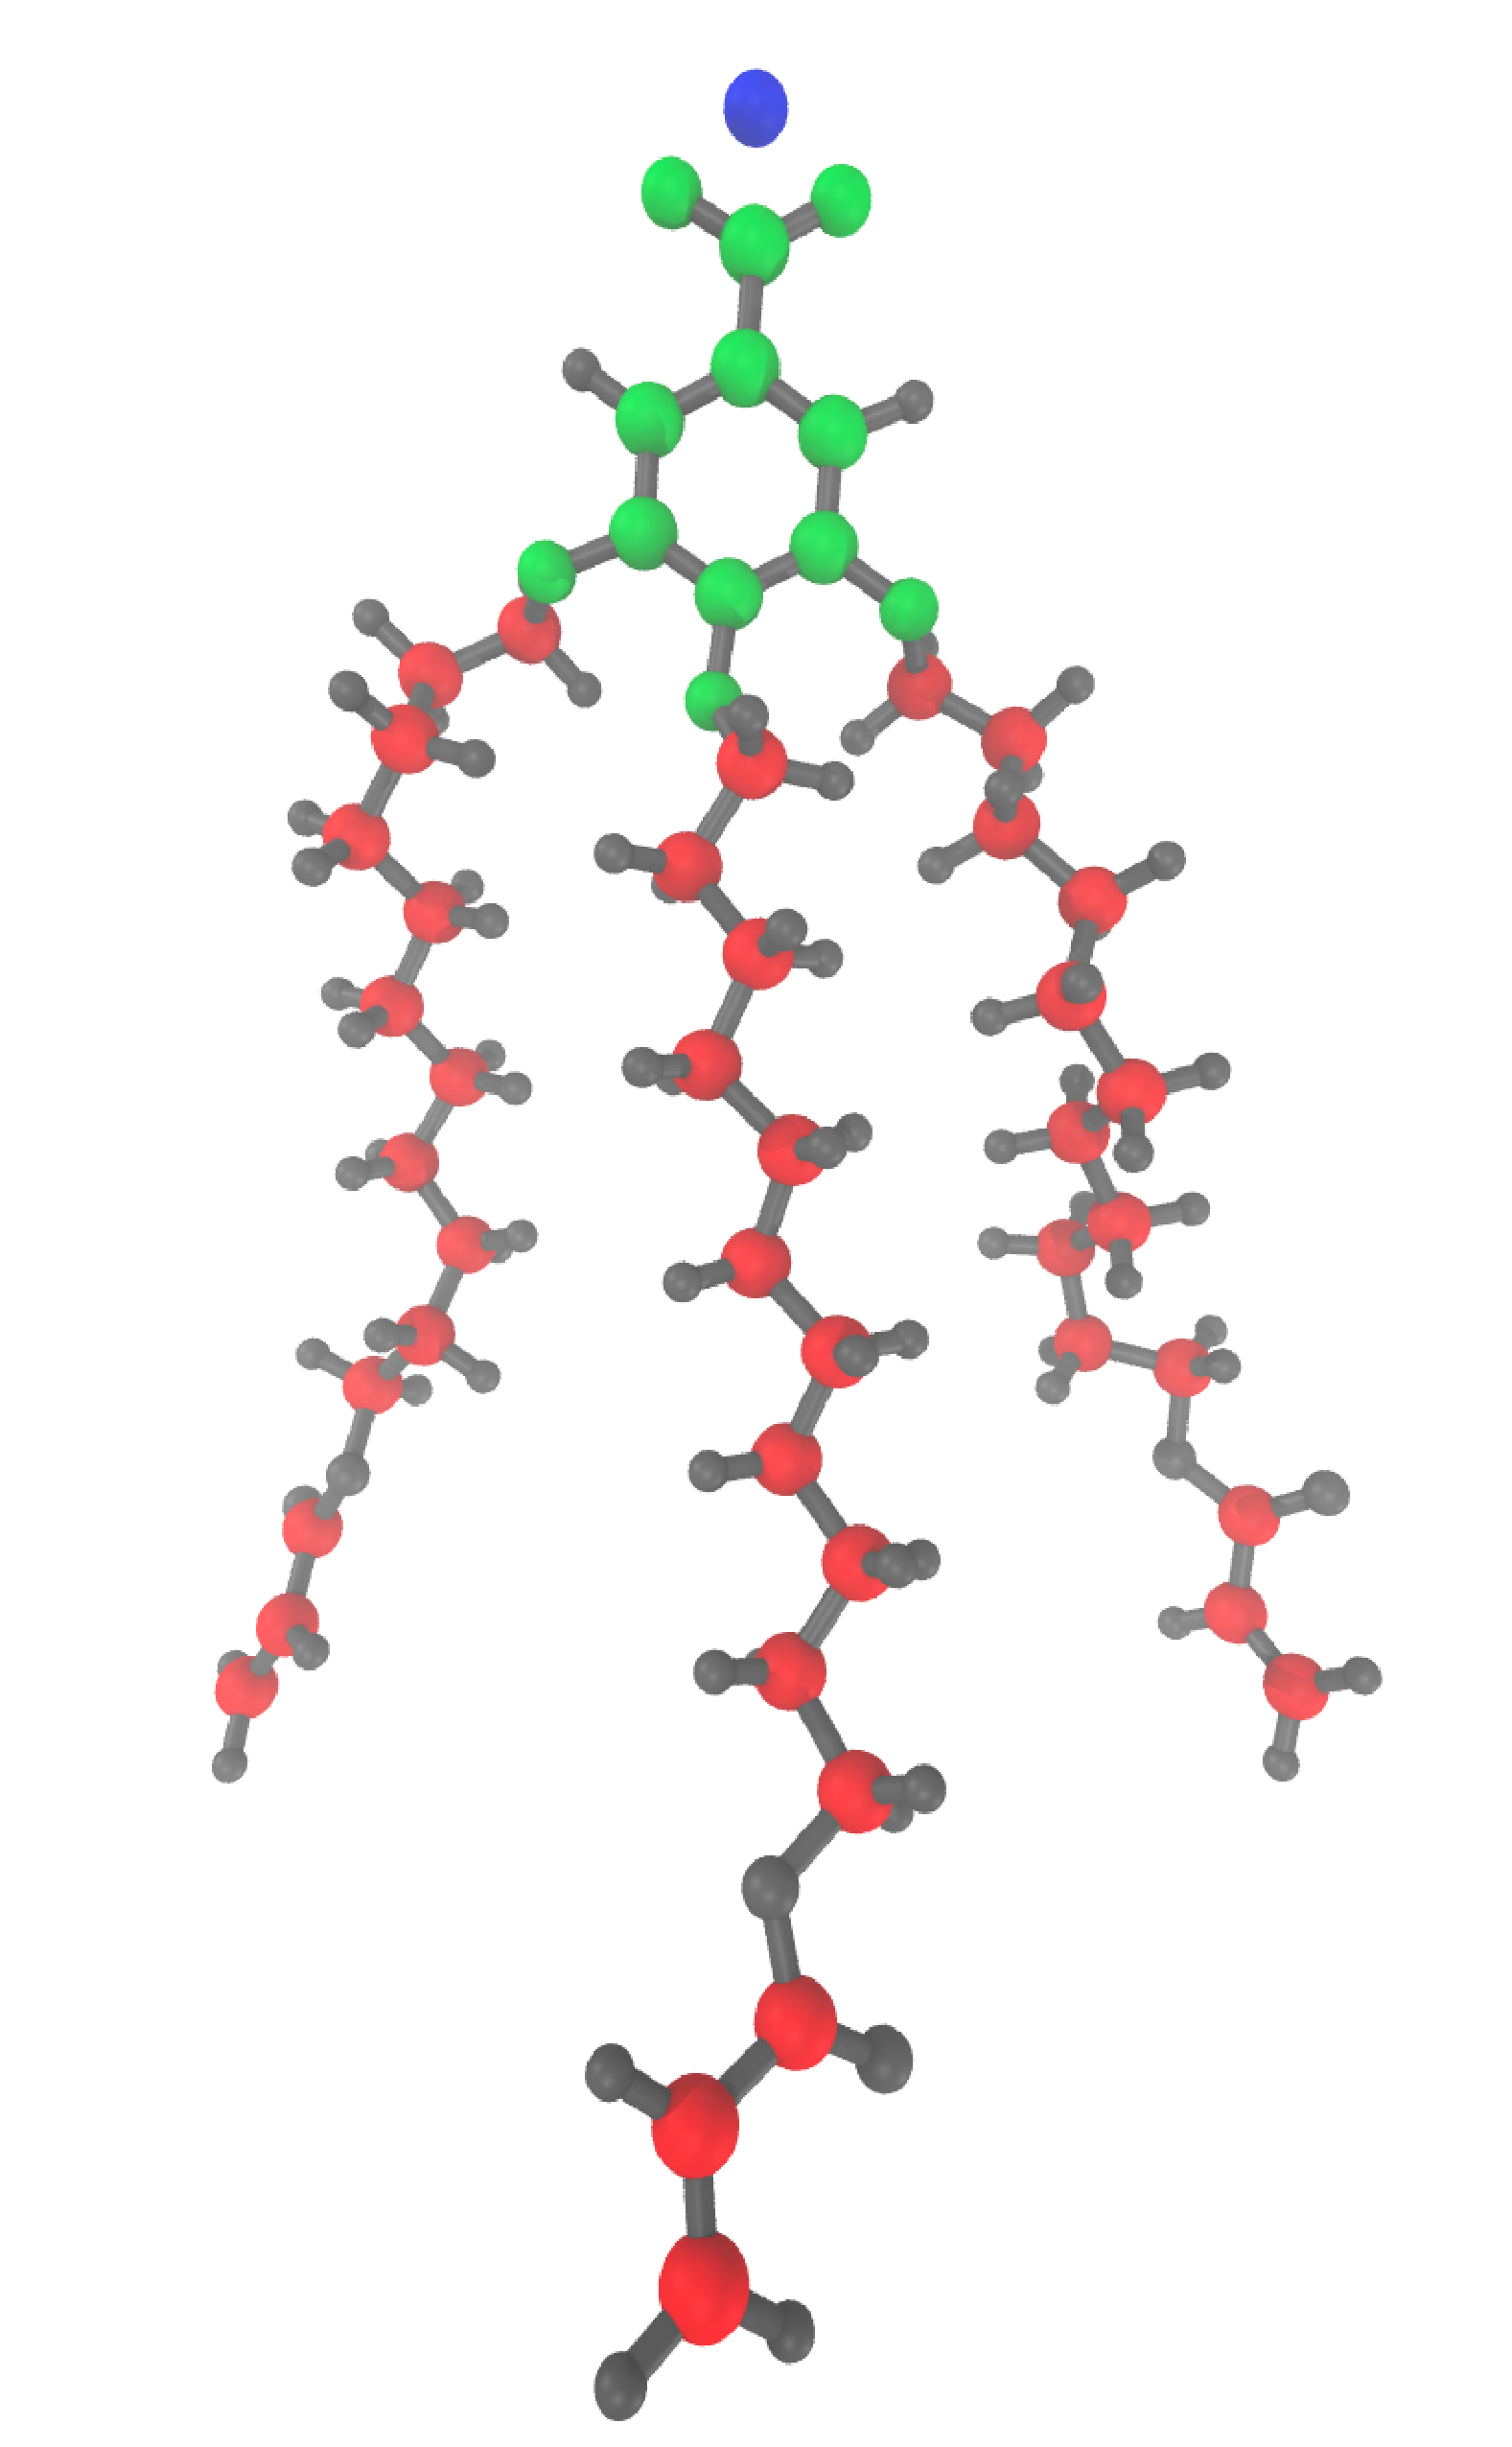
\includegraphics[width=\textwidth]{monomer_color_coded.pdf}
  \label{fig:monomer_color_coded}
  \end{subfigure}
  \begin{subfigure}{0.45\textwidth}
  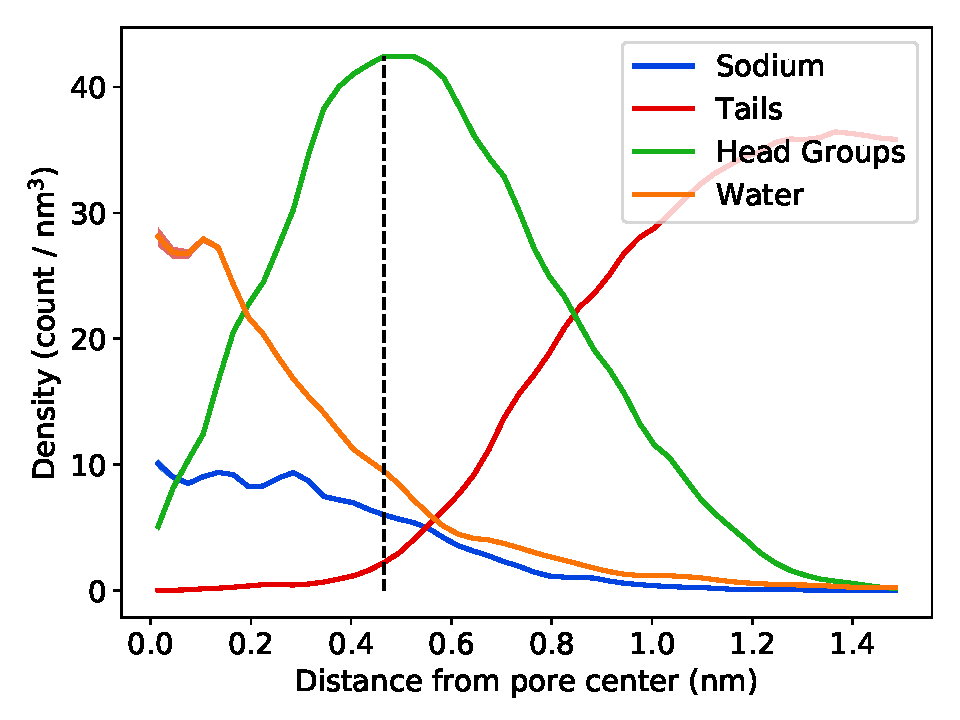
\includegraphics[width=\textwidth]{component_density_5wt.pdf}
  \caption{5 wt\% water}\label{fig:component_density_5wt}
  \end{subfigure}
  \begin{subfigure}{0.45\textwidth}
  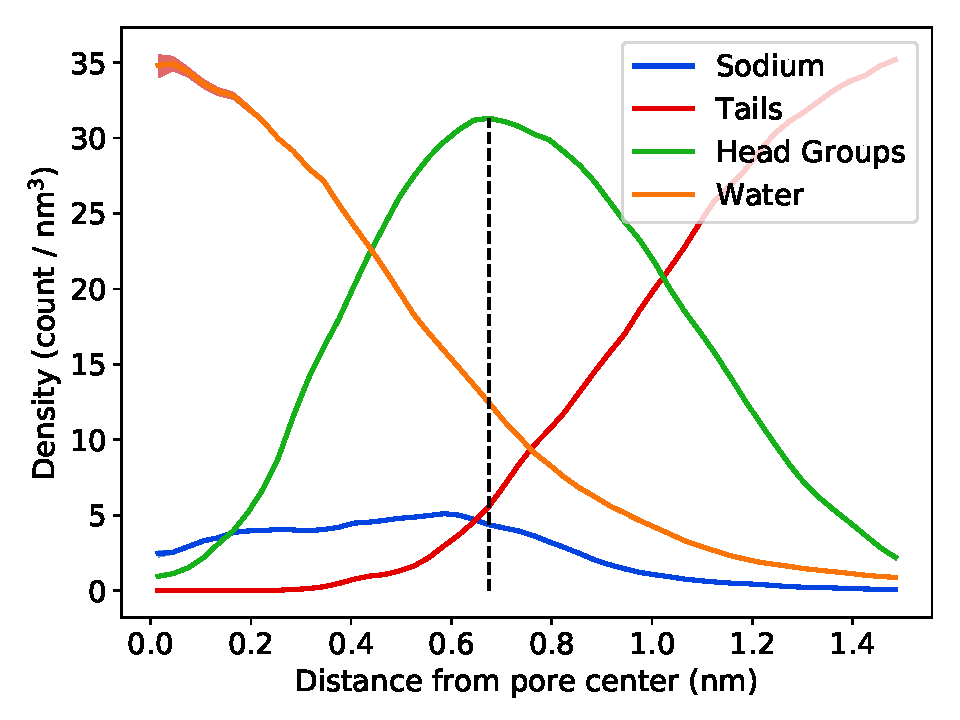
\includegraphics[width=\textwidth]{component_density_10wt.pdf}
  \caption{10 wt\% water}\label{fig:component_density_10wt}
  \end{subfigure}
  %MRS2: interesting that the head group max is near the transition point where water/tail groups 
  \caption{The radial densities of various monomer components paint a 
  picture of the pore topology where the pore centers of hydrated systems are primarily,
  but not exclusively, composed of water and sodium ions. The monomer groups labeled in each plot correspond to 
  the color-coded monomer pictured in the upper right corner of the figure. 
  RDFs show the average number of atoms located at a given distance from the
  pore center normalized by the volume of the annular bin to which they belong.
  The vertical dashed black lines are positioned so that they intersect with 
  the maximum head group density.
  (a) In the dry system, the density of head groups and sodium ions are highest
  0.15 to 0.4 nm from the pore center. There is an appreciable density of head groups
  crowding the pore center. (b) In the 5 wt\% system, monomer head 
  groups retreat radially in order to make room for water molecules at the pore center.
  (c) Monomers in the 10 wt\% system retreat an additional 0.2 nm to make room
  for more water.}\label{fig:component_densities}
  \end{figure}
  
  %MRS2: probably would be better to consolidate the information about water in the tails in one place.  Could be here?
  %MRS2: fundamentally, needs to be explicit justification of the choice to look at transport in the pores alone.

  There is an appreciable amount of water that partitions into the distal tail
  region of both systems. 28\% and 31\% of the total water is present in the
  distal tail regions of the 5 and 10 wt\% water systems respectively. See 
  Section~\ref{S-section:water_content_equil} of the Supporting Information 
  for more details on the equilibrations that led to this conclusion. The partition
  is due to a combination of the distal tail region's lower density as well
  as oxygen atoms at the ends of each monomer tail which can further stabilize
  water molecules. See Figure~\ref{S-fig:total_density} of the Supporting 
  Information for a graphical illustration of this point.
  
  We will restrict our studies of transport to solutes and water outside of the 
  distal tail region because transport is fastest in the pores. We provide more 
  rigorous justification for this restriction at the end of Section~\ref{section:transport_water_sodium}.

  \subsection{Mechanisms Governing Small Solute Transport}\label{section:mechanism_overview} 

  We observed transport of sodium, water and 20 other small polar solutes
  inside the membrane nanopores. First, we comment on transport of the
  membrane constituents, water and sodium, in a system absent of any additional
  solutes. We then present the general trends that we observe among the
  all other solutes studied.
  
  \subsubsection{Water and Sodium Ions}\label{section:transport_water_sodium} 

  Water and sodium's mobilities increase in larger and less crowded pores. 
  In the 10 wt\% water system, the MSD of water is about 51 times higher and
  the MSD of sodium is about 49 times higher compared to the 5 wt\% water system. 
  In the 10 wt\% water system, water moves about 51 times faster than sodium 
  and in the 5 wt\% system, water moves about 49 times faster than sodium. Due to
  the linearity of water's MSD in the 10 wt\% water system, we assumed
  long timescale Brownian behavior and measured its diffusivity to be 
  $7.45 \times 10^{-7}$cm$^2$/s which is only 1.4\% that of bulk TIP3P 
  water.~\cite{mahoney_diffusion_2000} %BJC: 7.45e-07 versus 5.19e-05 cm^2/s
  
  % Plots generated with msd_curves.py in figures folder
  % BJC: I show up to 400 ns time lag. Any reason to show full 1000 ns?
  \begin{figure}[!htb]
  \centering
  \begin{subfigure}{0.45\textwidth}
  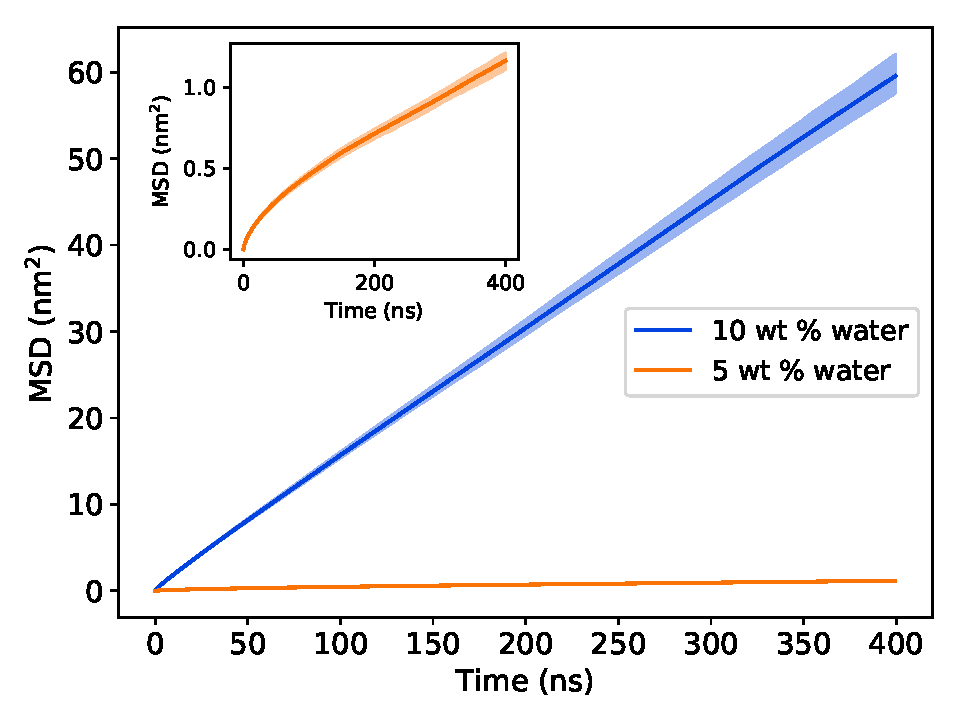
\includegraphics[width=\textwidth]{water_msd_comparison.pdf}
  \caption{Water}\label{fig:water_msd_comparison}
  \end{subfigure}
  \begin{subfigure}{0.45\textwidth}
  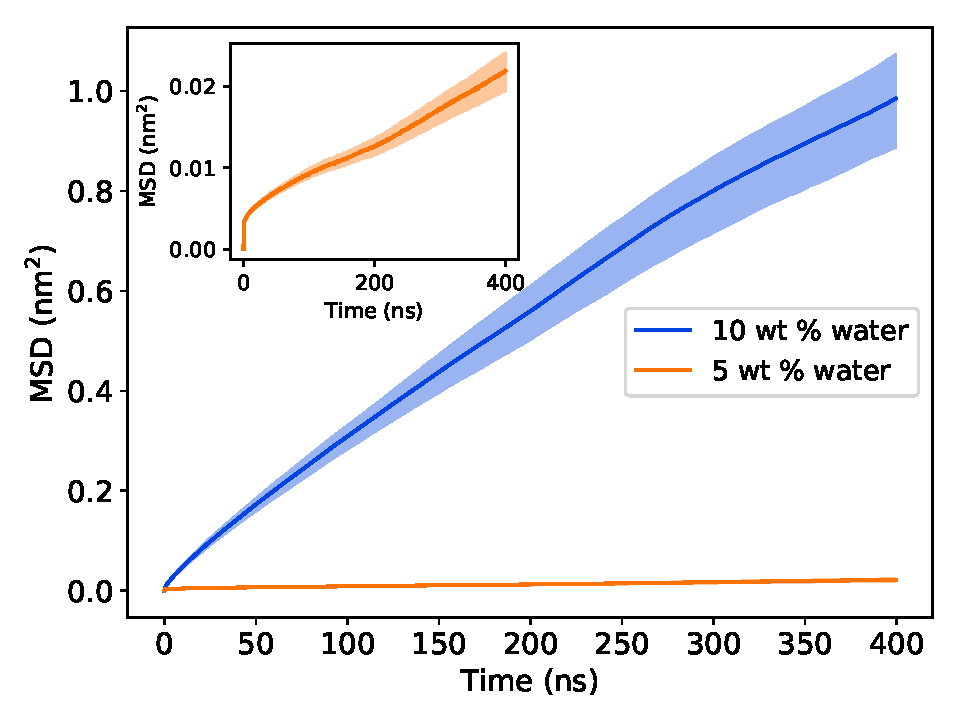
\includegraphics[width=\textwidth]{na_msd_comparison.pdf}
  \caption{Sodium Ions}\label{fig:na_msd_comparison}
  \end{subfigure}
  \caption{(a) The $z$-direction MSD of water in the 10 wt\% water system 
  is about 51 times higher than water in the 5 wt\% water system. Water 
  appears to exhibit Brownian motion in the 10 wt\% system due to its
  linear MSD. (b) The MSD of sodium in the 10 wt\% water system is about 
  49 times higher than sodium in the 5 wt\% water system.}\label{fig:msd_comparison}
  \end{figure}

  Sodium coordinates with both water and carboxylate moieties from the head
  groups in the pores. Sodium coordinates with 3.4 water molecules in bulk 
  solution (see Section~\ref{method:coordination}), but on average in the pores,
  coordinates with 1.7 water molecules in the 10 wt\% system and 1.2 water
  molecules in the 5 wt\% system. The sodium ions additionally coordinate with
  1 carboxylate group in the 10 wt\% water system and 0.8 carboxylate groups 
  in the 5 wt\% water system. This behavior likely slows the motion of the 
  sodium ions considerably compared to bulk water.
  %MRS2: is one sodium per carboxylate group correct?
  %BJC3: yes, if sodium within cutoff of both oxygens, it is only counted once.
  % Assuming only one sodium per carboxylate group, the numbers were multiplied by 2
  % since the averages were divided by 800 instead of 400

  In the 10 wt\% water system, water molecules that spend the majority of 
  their time in the distal tail region move significantly slower than those
  close to the pore center. In Figure~\ref{fig:water_msd_comparison}, we 
  constructed the MSD curves based on water molecules that spent $>$ 95\% of their
  time outside the distal tail region. If we instead restrict our calculation to
  water molecules that spend $>$ 95\% of their time \textit{in} the distal tail region, 
  the MSD of water is about 8 times lower, decreasing from 59.6 to 8.2 nm$^2$. 
  
  % Changing pore radius does not change conclusion here.
  In the 5 wt\% water system, water molecules that spend the majority of their 
  time in the distal tail region have MSDs slightly higher than those of water molecules
  close to the pore center. The MSD of distal tail water molecules is 1.7 nm$^2$
  compared to 1.2 nm$^2$ outside the distal tails. This anomaly is likely a 
  consequence of lower density in the distal tails relative to the pores,
  leading to faster diffusion in the tails,
  as well as slowed diffusion of water molecules in the pores via hydrogen bonds
  with other water molecules and association with sodium ions. Water molecules 
  are less likely to hydrogen bond with each other while in the distal tail 
  region since they are interspersed between chains, while those in 
  the pores stay in close proximity to each other. We observed about 9 times more  % tailvpore_hbonding.py in figures folder
  hydrogen bonding between water molecules near the pore center versus those in 
  the distal tail region. Additionally, an average of 65\% of water molecules in
  the pores of the 5 wt\% water system are associated with a sodium ion each frame
  compared to 44 \% in the 10 wt\% water system. There is a negligible amount of
  hydrogen bonds between water molecules and monomer head groups. 
  
  Because the MSD of water in the pores of the 10 wt\% system is significantly
  higher than that in the tails, we restrict our studies of transport in this paper to 
  solutes in or near the pore center. Transport of solutes in the pores 
  %MRS3:
  %will 
  is likely to be
  be the 
  limiting factor that determines permeability and rejection. Although tail transport of water in the 
  the 5 wt\% water system is faster than pore transport, water transport overall is significantly slower
  than in the 10 wt\% system. For practical applications, a membrane with water 
  transport properties comparable to the 10 wt\% system is far more feasible than
  the 5 wt\% system.
 
%  45 \% of water molecules associated with sodium in 5 wt\% system
%  
%  While a similar observation holds for the 10 wt\% system,
%  its high water content facilitates a less crowded environment where diffusion
%  of water molecules dominates.  
%  %MRS4: math seems a little inconsistent.  Does the tail water move the same rate in 5 and 10%? Seems like it should.
%  %MRS4: but above would tend to indicate that it moves 51/8 = 6.4 times faster in the tails in 10%? 
%  %MRS4: think about reading over/describing the tail water here
%  %MRS4: would probably be useful to the reader to specify that we are neglecting transport in the tails here.
%
%  Hydrogen bonds to charged things. Dipole-point charge stronger than dipole-dipole
%  Quantify water 
%
%  10 wt will be the only practical membrane.
%
%  Set up simulations with high percent methanol

 \subsubsection{Transport of Small Polar Solutes}\label{section:general_transport_solutes}  
  
  We observe trends in transport properties that are dependent on the chemical 
  environment within the nanopores rather than just solute size. Polar solutes
  are slowed by interactions between monomer functional groups and ions. 
  A thorough understanding of these interactions will help us to create monomer
  design principles. We will begin our analysis by considering the collective
  trends observed across all systems and then focus on subsets of molecules
  with structural similarities.

  As with water and sodium, the MSDs of the solutes studied in this work are 
  significantly larger in the 10 wt\% system than those in the 5 wt\% water 
  system (see Figures~\ref{fig:all_msds_5wt} and~\ref{fig:all_msds_10wt}). The fastest moving solute in both cases, 
  methanol, has an MSD about 175 times larger in the 10 versus the 5 wt\%
  water system. Clearly the equilibrium water content of a given LLC system will 
  determine its viability for real separations.
  
  The MSDs are not solely a function of solute size. We plotted each solute's radius
  against their MSD in Figures~\ref{fig:msd_radius_5wt} and~\ref{fig:msd_radius_10wt}.
  Of all the solutes, methanol is likely subject to the least hindrance by
  the membrane due its small size. Therefore we fit Equation~\ref{eqn:msd-stokes-einstein}
  so that it intersects with methanol's average MSD and radius. The uncorrected version of 
  Equation~\ref{eqn:msd-stokes-einstein} ($f$=1) is plotted and converges to the same value as the
  corrected form for large radii (see Section~\ref{method:stokes}). Although both curves are 
  approximations, they illustrate that the majority of solutes in our study show
  lower than expected MSDs. In most cases, the predicted MSDs even fall below the 
  conservative uncorrected Stokes-Einstein estimate. It is clear that more complex
  mechanisms determine the MSDs of these solutes.
  
  \begin{figure}[!htb]
  \centering
  \begin{subfigure}{0.45\textwidth}
  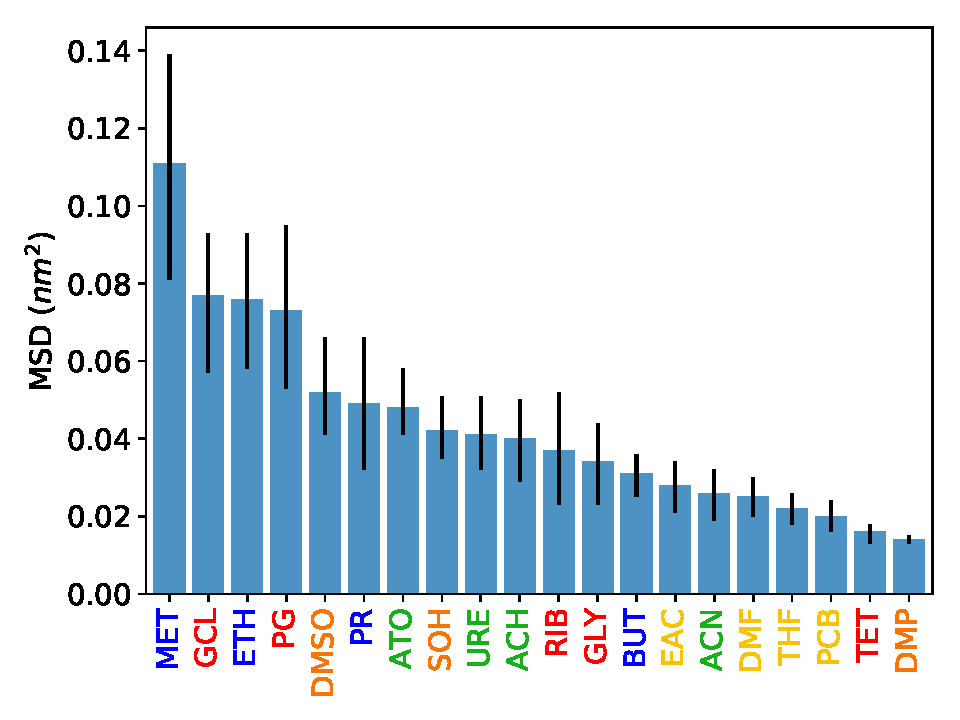
\includegraphics[width=\textwidth]{all_5wt_tamsds.pdf}
  \caption{5 wt\% water}\label{fig:all_msds_5wt}
  \end{subfigure}
  \begin{subfigure}{0.45\textwidth}
  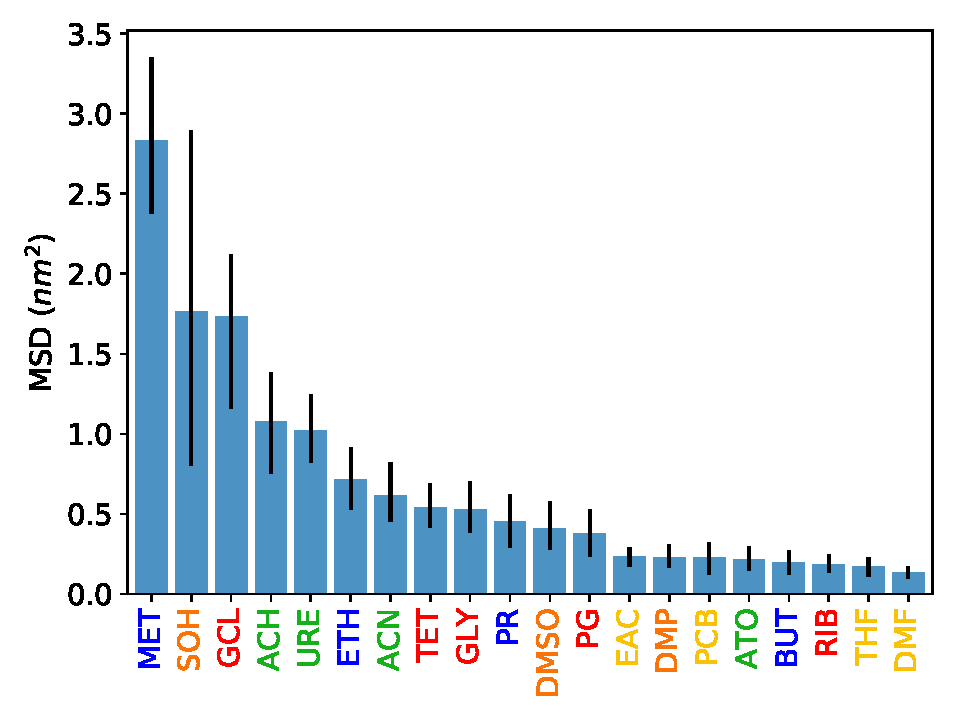
\includegraphics[width=\textwidth]{all_10wt_tamsds.pdf}
  \caption{10 wt\% water}\label{fig:all_msds_10wt}
  \end{subfigure}
  \begin{subfigure}{0.45\textwidth}
  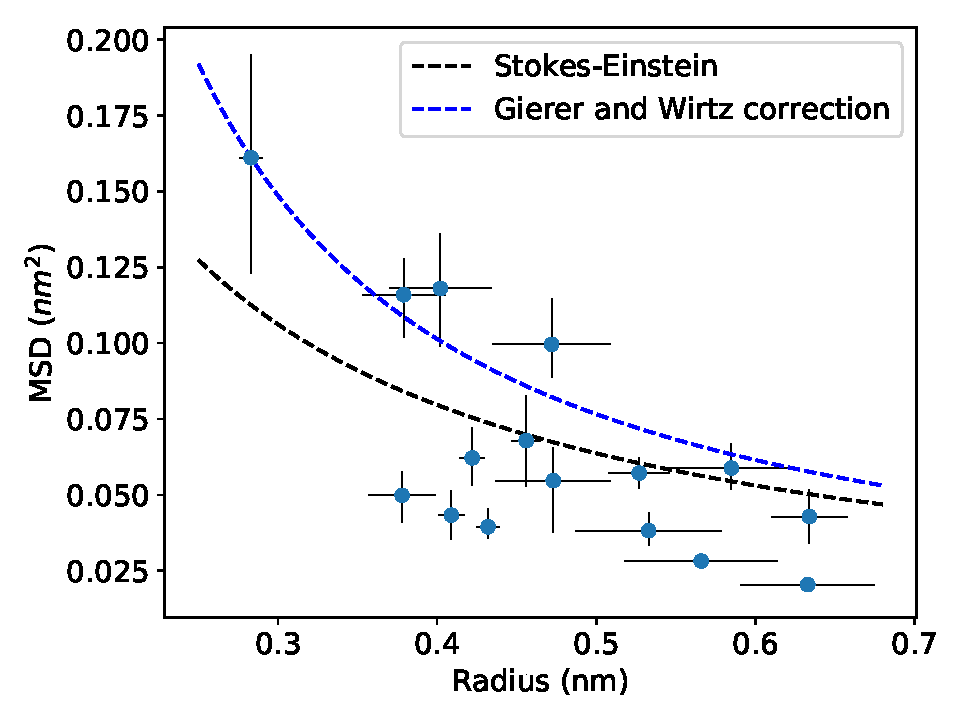
\includegraphics[width=\textwidth]{msd_radius_5wt.pdf} 
  \caption{5 wt\% water}\label{fig:msd_radius_5wt}
  \end{subfigure}
  \begin{subfigure}{0.45\textwidth}
  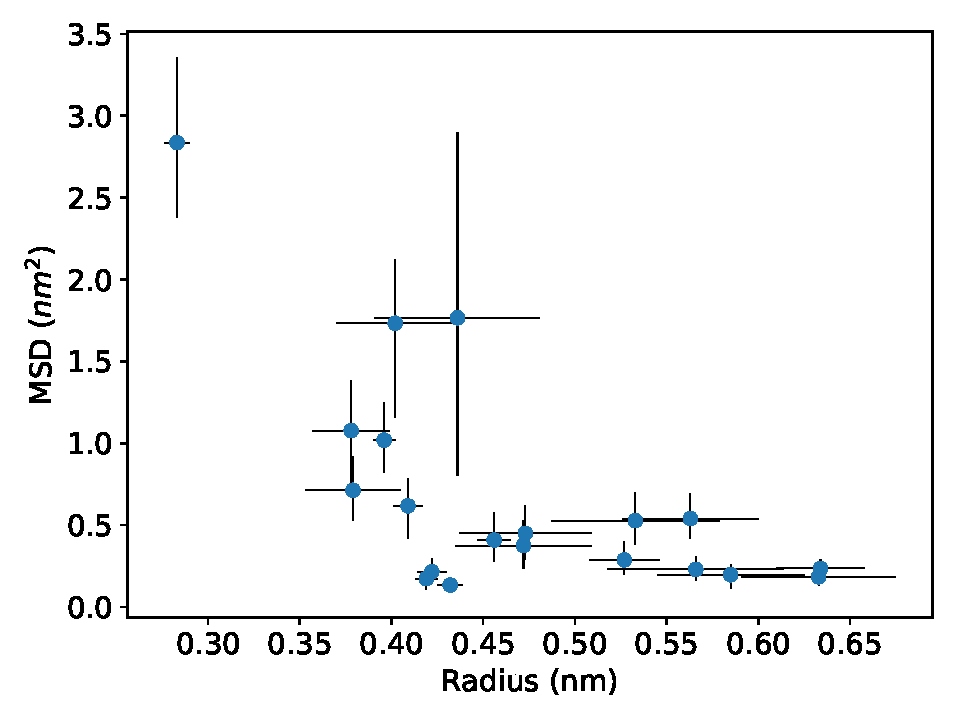
\includegraphics[width=\textwidth]{msd_radius_10wt.pdf} 
  \caption{10 wt\% water}\label{fig:msd_radius_10wt}
  \end{subfigure}
  %MRS2: should an explicit note of the change of scale from 5% to 10% graph; easiest is in the caption.  Could also note it by some
  %MRS2: some sort of graphical indication on the graph itself.  But definitely need to draw attention to it. 

  \caption{The MSDs of solutes in the 5 wt\% water system (a) are significantly
  smaller than those of the solutes in the 10 wt\% water system (b). The
  MSDs are not a monotonic function of molecular size (c and d). A significant
  number of solute MSDs fall below the theoretical lines predicted by the 
  Stokes-Einstein equation and Gierer and Wirtz' corrected Stokes-Einstein equation.
  }\label{fig:msds}
  \end{figure}
    
  On the timescales simulated in our study, solutes exhibit subdiffusive
  behavior. Figure~\ref{fig:example_ztraces} plots the $z$-coordinate versus
  time of 3 representative ethanol centers of mass in the 10 wt\% water system.
  There are clear periods of entrapment separated by relatively large hops.
  The MSD calculated based on all ethanol molecules is plotted in 
  Figure~\ref{fig:example_msd} and its shape is sublinear. The long periods
  of entrapment lead in part to this sublinear, and thus subdiffusive, behavior.
  
  \begin{figure}[!htb]
  \centering
  \begin{subfigure}{0.49\textwidth}
  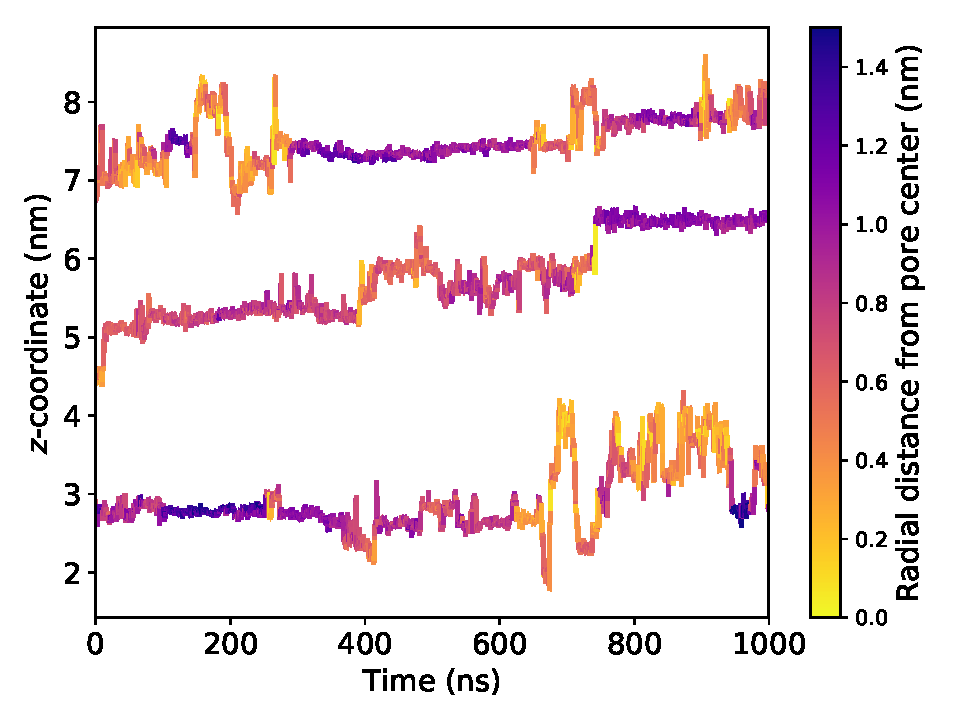
\includegraphics[width=\linewidth]{colorful_example_ztraces.pdf}
  \caption{}\label{fig:example_ztraces}
  \end{subfigure}
  \begin{subfigure}{0.49\textwidth}
  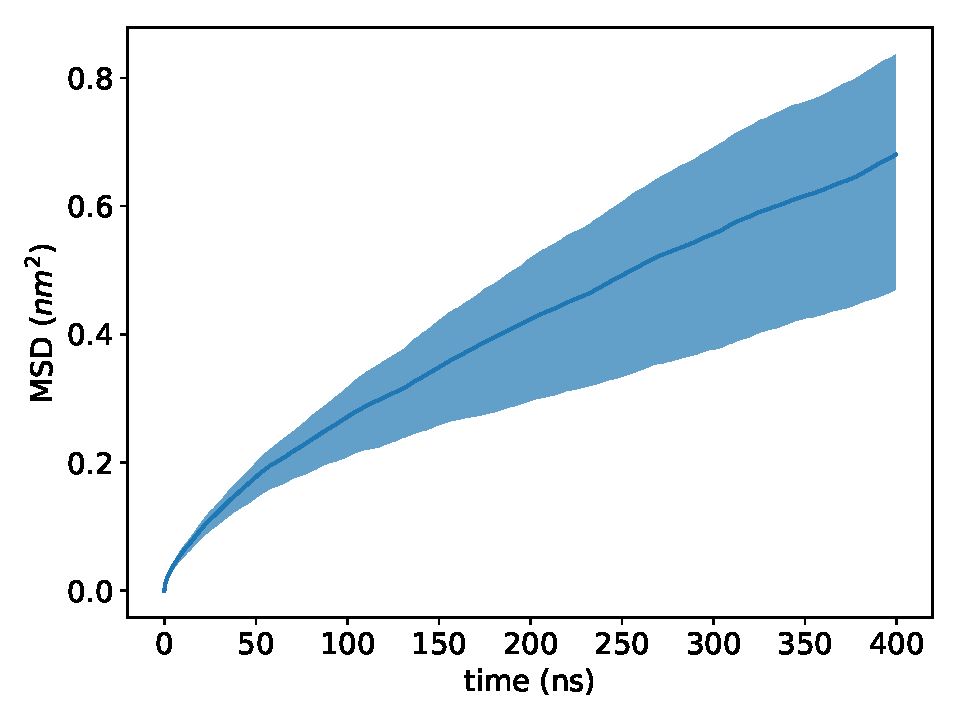
\includegraphics[width=\linewidth]{example_msd.pdf}
  \caption{}\label{fig:example_msd}
  \end{subfigure}
  \caption{All solutes show subdiffusive transport behavior inside the membrane's
  nanopores, similar to that exhibited by ethanol. (a) The $z$-coordinate trace of
  3 representative ethanol COMs shows clear periods of entrapment separated by hops.
  In general, the longest dwell times occur when solutes are situated far from the
  pore center and more frequent hops occur when solutes are close to the pore center.
  (b) The time-averaged MSD of ethanol is sublinear which suggests transport is
  governed by an anomalous subdiffusion process.}\label{fig:qualitative_mechanisms}
  \end{figure}
  
  The complex and non-homogeneous structure of the membrane leads to radially
  dependent transport mechanisms. In general, we observed that hops 
  made in the pore region are about 59\% larger than those made outside
  the pore region (see Figure~\ref{fig:hop_lengths}). There is a high 
  resistance to movement in the alkane-dense head group and tail regions
  while, in the pore region, solutes can move relatively freely since it 
  is primarily composed of water molecules. However, time spent in the 
  pore region does not necessarily lead to more frequent hopping. The 
  largest solutes in this study spend the most time in the pore region
  (see Figure~\ref{fig:frac_time}), but many hop with a below-average
  frequency (see Figure~\ref{fig:hopfreq}). Therefore, trapping mechanisms
  controlled by membrane properties other than alkane density must be prevalent.

%  Solutes partition out of the pore into the head group region and beyond
%  which may lead to a radially dependent transport mechanism. It is clear 
%  from Figure~\ref{fig:example_ztraces} that the longest periods of 
%  entrapment usually occur when solutes are far from the pore center.
 
  % When hops occur, and where there is the most $z$-positional
  % noise, solutes are generally close to the pore center  

  \begin{figure}
  \centering
  \begin{subfigure}{0.325\textwidth}
  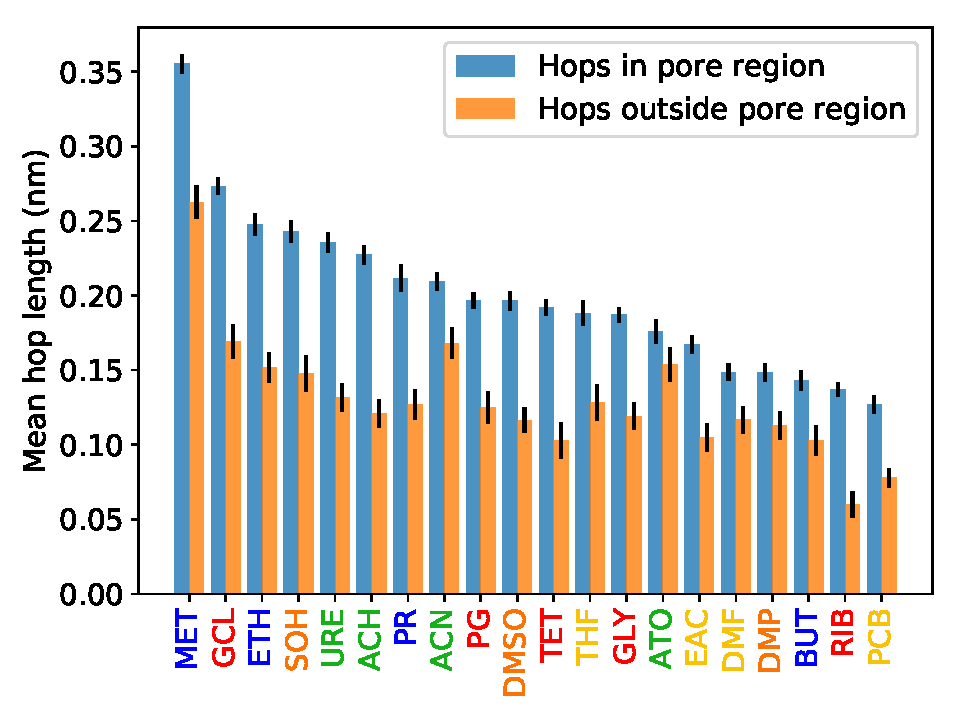
\includegraphics[width=\linewidth]{hop_length.pdf}
  \caption{}\label{fig:hop_lengths}
  \end{subfigure}
  \begin{subfigure}{0.325\textwidth}
  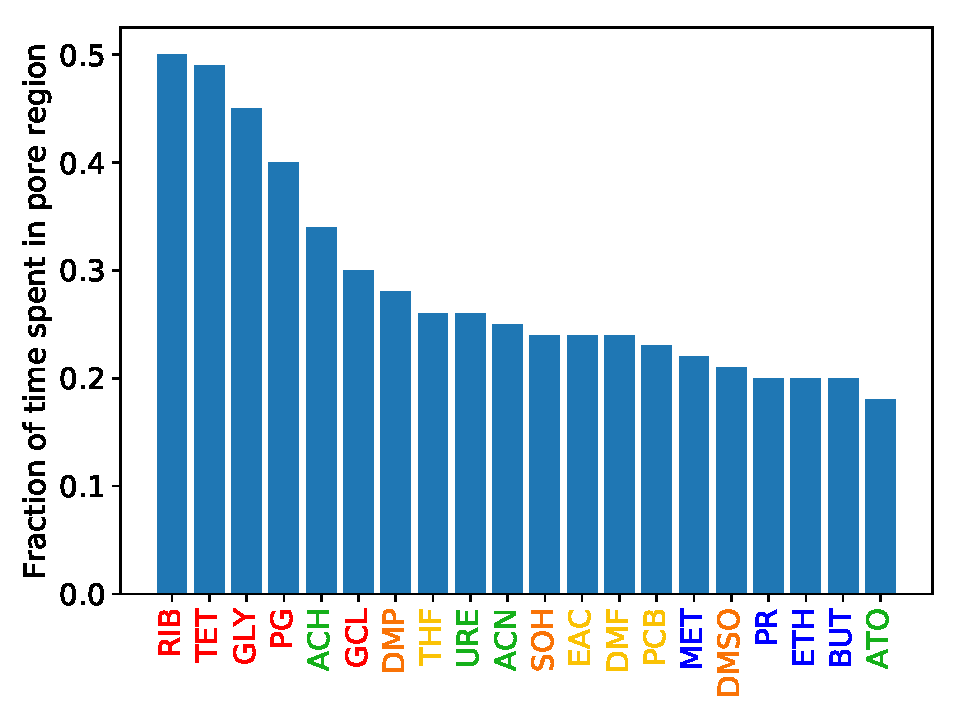
\includegraphics[width=\textwidth]{frac_time_spent.pdf}
  \caption{}\label{fig:frac_time}
  \end{subfigure}
  \begin{subfigure}{0.325\textwidth}
  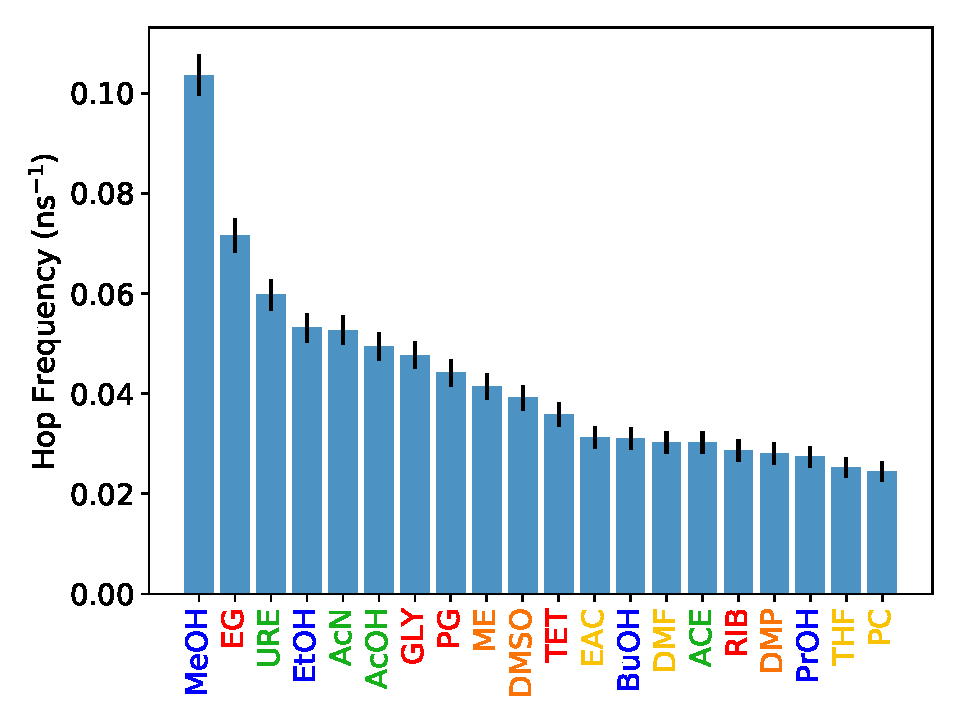
\includegraphics[width=\textwidth]{hopfreq_total.pdf}
  \caption{}\label{fig:hopfreq}
  \end{subfigure}
  \caption{(a) Hops made in the pore region of the 10 wt\% water system 
  are, on average, 59\% larger than those made outside the pore region. 
  The trend in hop lengths is similar to the trend in MSDs shown in 
  Figure~\ref{fig:all_msds_10wt} implying that solutes which make consistently 
  larger hops have higher MSDs. The fraction of time spent by a solute in the 
  pore region (b) does not necessarily lead to more frequent hopping (c). For
  example, ribose spends the largest fraction of time in the pore region, yet
  hops the fifth least frequently.}\label{fig:hops}
  \end{figure}
  
  %In addition to solute trapping in dense monomer regions, 
  We observe a second trapping mechanism caused by preferential hydrogen 
  bonding between hydrogen bond donor solutes and monomer head groups. To 
  continue with our ethanol example, we observe that 64\% of ethanol 
  molecules donate hydrogen bonds  % 15.7/24 donated, 0.6/24 accept -- BJC: double check these numbers
  and 3\% of ethanol molecules accept hydrogen bonds each frame. On average, 40\%
  of hydrogen bonds donated by ethanol go to carboxylate % BJC1: 6.33 hbonds between EtOH and COOH per frame, 3.84 b/w EtOH and ether oxygen, 5.56 between EtOH and HOH (where Ethanol donates)
  head groups, 25\% go to the ether linkages connecting the monomers tails to the 
  head groups and the remaining 35\% to water. There are about 46\% less  % 800 carboxylate oxygens total versus 2158 * 0.69 total water molecules in pores 
  carboxylate oxygen atoms in the pore than there are water molecules yet more
  hydrogen bonds are donated to them. The stability of hydrogen bonds with 
  carboxylate oxygen atoms is high because they have a negative charge
  with no neutralizing positive charges nearby. Additionally, on average, 
  each sodium ion is coordinated to 1.7 water molecules meaning an appreciable
  fraction of the water molecules occupying the pore region are usually 
  coordinated to a sodium ion which decreases their availability to accept 
  hydrogen bonds from solutes.
  % MRS1: this should lead to reduced ability to solvate positive things, but 
  % shouldn't reduce H-bonding that much?
  % BJC1: I think that it takes away acceptor oxygen atoms since they are occupied
  % by sodium. The hydrogen atoms of water could still hbond but I'm just talking
  % about ethanol donating to water's oxygen, for which opportunities should be suppressed.
  
  The lifetime of hydrogen bonds between solutes and monomer head groups tends to 
  be longer for solutes that hydrogen bond more frequently. In Figure~\ref{fig:hbonds}
  we see nearly the same ordering of the percentage of solutes hydrogen bonded to
  monomer head groups and the 95\textsuperscript{th} percentile of hydrogen bond 
  lifetimes. Solutes with multiple hydroxyl groups donate hydrogen bonds most 
  frequently and tend to stay hydrogen bonded longer. Hydrogen bonds donated by
  nitrogen are far less common and tend to be short-lived as shown by acetamide
  and urea.

  \begin{figure}[!htb]
  \centering
  \begin{subfigure}{0.45\textwidth}
  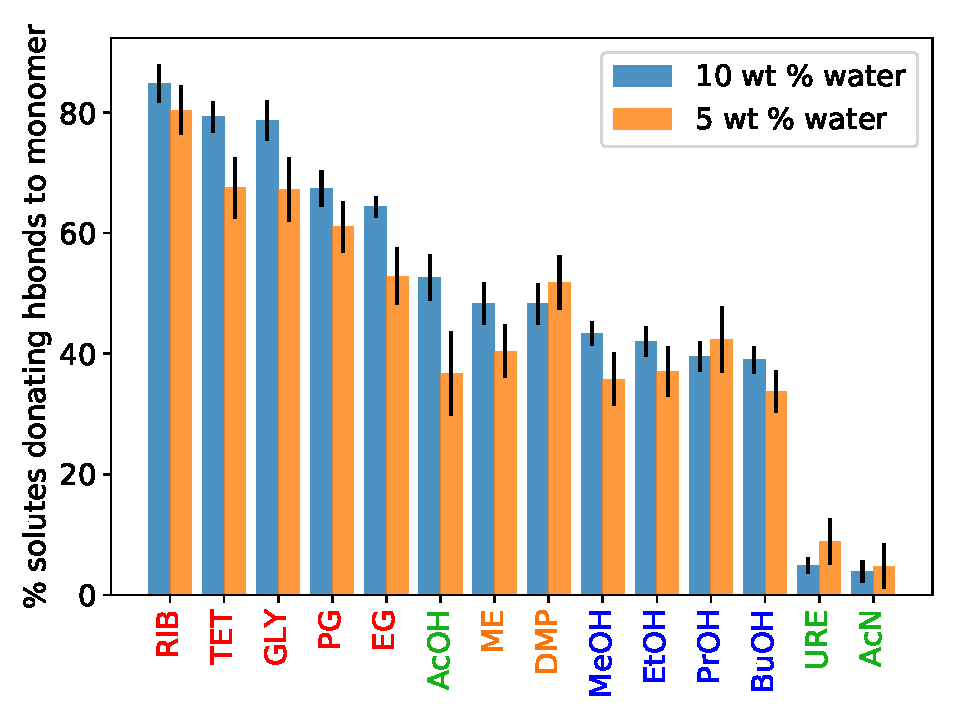
\includegraphics[width=\textwidth]{nhbonds_all.pdf}  % unique_hbonds.py
  \caption{}\label{fig:nhbonds}
  \end{subfigure}
  \begin{subfigure}{0.45\textwidth}
  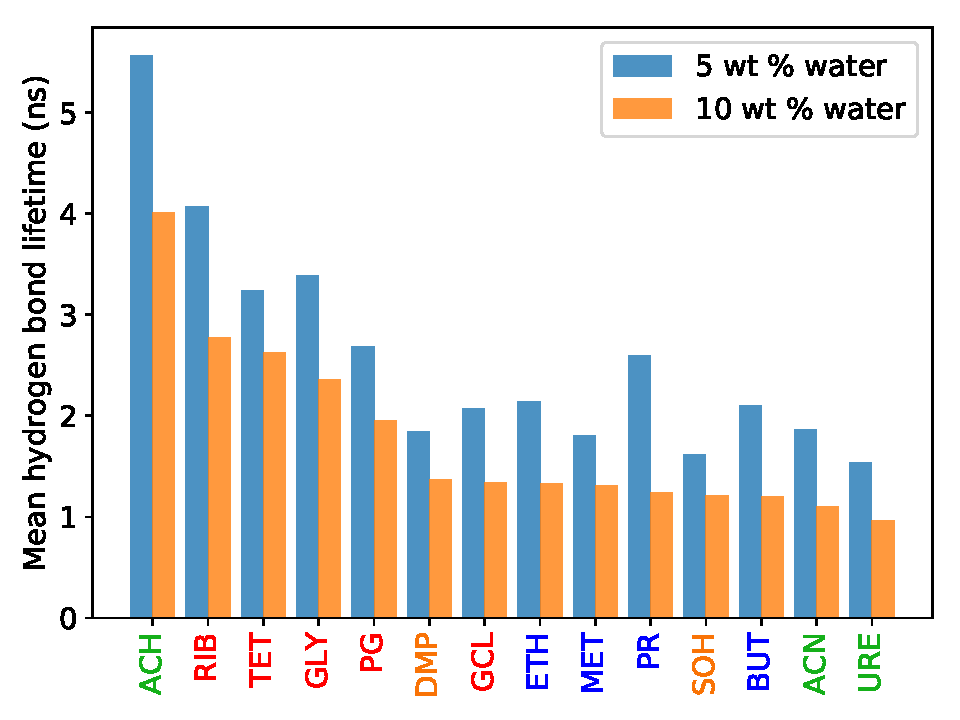
\includegraphics[width=\textwidth]{hbond_lifetime.pdf}  % hbond_dwells.py
  \caption{}\label{fig:hbond_dwells}
  \end{subfigure}
  \caption{(a) Solutes capable of donating hydrogen bonds to monomer head groups
  do so to varying degrees. The reported percentages represent unique solute-monomer
  hydrogen bonds. Individual solutes that hydrogen bond with multiple head groups
  simultaneously are only counted once. (b) The lifetime of individual hydrogen
  bonds appears correlated to the percentage of solutes involved in hydrogen bond
  interactions. Hydrogen bond lifetimes tend to be longer for solutes that 
  hydrogen bond frequently. Note that solutes incapable of donating hydrogen
  bonds are omitted from this figure.}\label{fig:hbonds}
  \end{figure}
  
  Finally, we observe slowing or immobilization of solutes that associate with
  sodium counterions. Much like water, the polarity of the solutes creates 
  regions of high electron density, modeled using partial negative charges, 
  which are stabilized through electrostatic interactions with sodium ions. 
  In Figure~\ref{fig:na_coordination}, we've plotted the average percentage
  of solutes coordinated to a sodium ion each frame as well as the
  95\textsuperscript{th} percentile of sodium association lifetimes. The degree and length of 
  coordination between solutes and sodium in the 5 wt\% water system is higher
  in all cases than that in the 10 wt\% water systems. The crowded pores of 
  the 5 wt\% water system forces sodium ions in close proximity to solutes. 
  
  Carbonyl functional groups tend to associate with sodium the most. Nearly
  all of the most coordinated solutes contain a carbonyl group (except for 
  DMSO which has an analogous sulfinyl group). There is a significant
  drop in sodium ion association for solutes that do not contain carbonyl 
  groups or multiple hydroxyl groups to compensate. The corresponding association
  lifetimes follow a similar trend, however the association lifetimes of highly coordinated 
  solutes with multiple hydroxyl groups are generally lower since association
  between hydroxyl groups and sodium is apparently a weaker interaction. Carbonyl
  groups contain an exposed and highly electron-dense oxygen atom which interacts
  readily with sodium ions. Carbonyl groups with nitrogen substituents appear
  to interact with sodium more frequently than those with carbon substituents. 
  Acetone associates with sodium significantly less than urea and acetamide. 

%  The dwell times are power law 
%  distributed, which means that while many of these interactions are fleeting,
%  there is still a chance for very long periods of association to occur. For 
%  example, the longest period of coordination between acetone and sodium was
%  110 ns.
%  There are many cases, particularly when an electronegative atom is left unprotected,
%  in which polar groups bind to sodium ions for at least a short period of time. 

  % need to think a little more about this. Numbers get skewed by different numbers
  % of oxygen atoms per solute. For example, the carbonyl group of acetic acid
  % associates with sodium a lot, but the OH doesn't really. (28 % C=O versus 3 % COH)
  \begin{figure}[!htb]
  \centering
  % BJC: maybe I should normalize these to number of oxygen atoms?
  \begin{subfigure}{0.45\textwidth}
  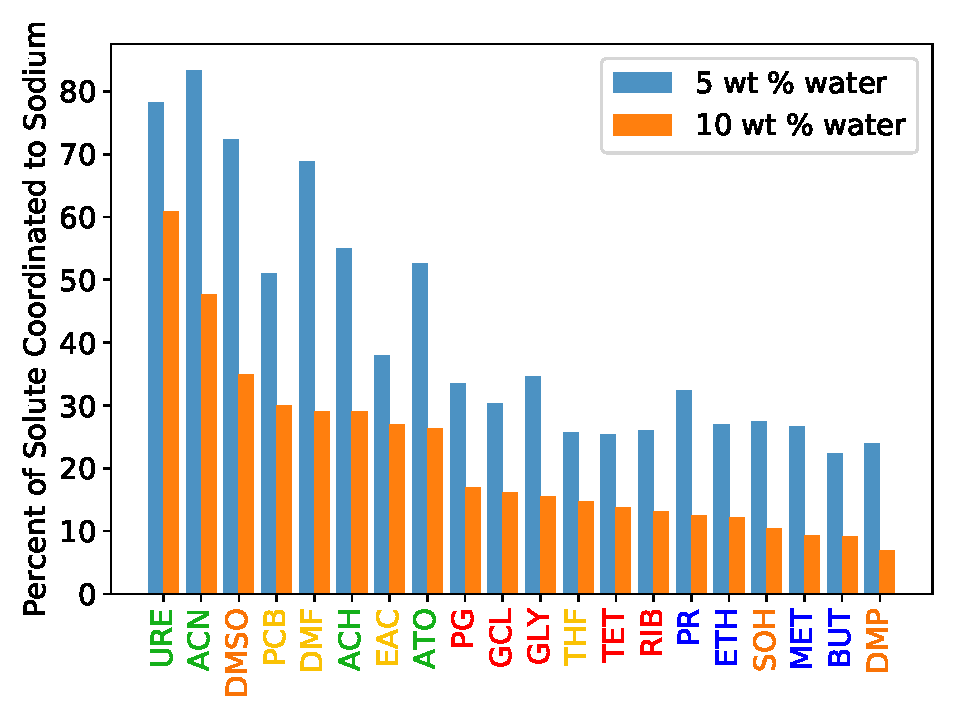
\includegraphics[width=\textwidth]{all_solutes_NA_coordination.pdf}  % all_coord.py
  \caption{}\label{fig:all_solutes_NA_coordination}
  \end{subfigure}
  \begin{subfigure}{0.45\textwidth}
  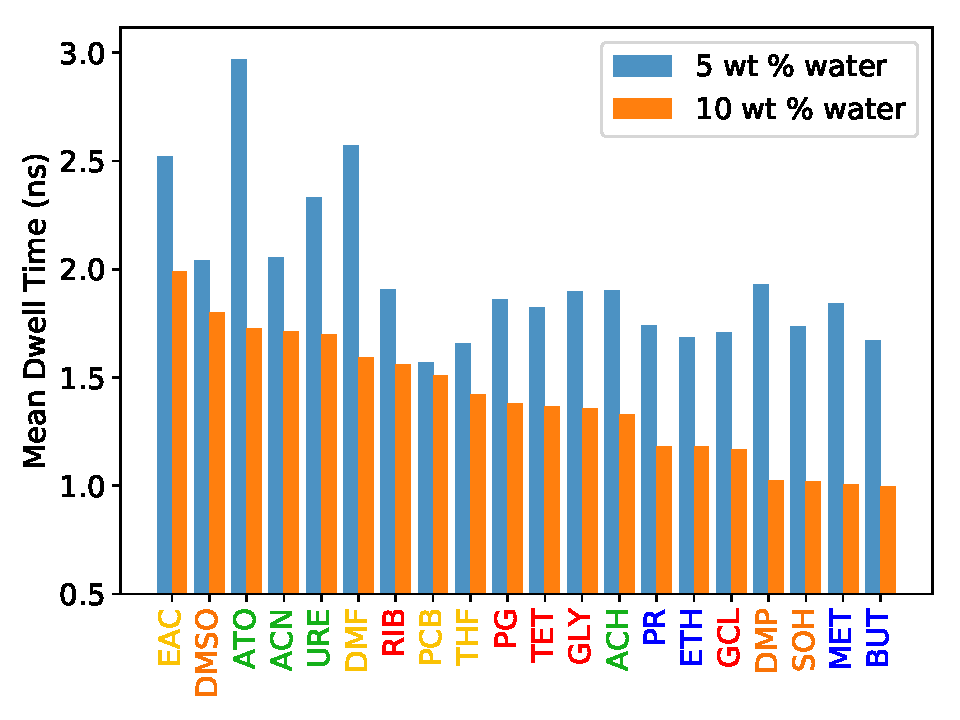
\includegraphics[width=\textwidth]{all_NA_dwells.pdf}  % na_dwells.py
  \caption{}\label{fig:all_NA_dwells}
  \end{subfigure}
  \caption{(a) Solutes, especially those with carbonyl groups, spend a 
  significant fraction of time coordinated to sodium ions. (b) The length
  of time a solute-sodium pairs spends associated tends to be higher for
  pairs that associate more frequently.}\label{fig:na_coordination}
  \end{figure}
  
  Coordination of ions with oxygen has been observed in a variety of systems. 
  Carvajal et al. noted that Na\textsuperscript{+} coordinated with four 
  THF molecules when they dissolved a sodium salt in the solvent.~\cite{carvajal_studies_1965}
  Wu et al. observed coordination of Na\textsuperscript{+} with the carbonyl
  group of a molecule used to design an organic electrode.~\cite{wu_unraveling_2015} 
  Finally, Shinoda et al. observed K\textsuperscript{+} ions coordinated with
  the carbonyl and hydroxyl groups of carboxy-terminal groups in crystallized
  ATPase.~\cite{shinoda_crystal_2009}
  
  Overall, the transport behavior exhibited by solutes in the 5 wt\% water
  systems is similar to that shown by those in the 10 wt\% system; however
  the timescales are much longer. We observe subdiffusive behavior with 
  intermittent hopping between periods of entrapment and evidence
  of the same three trapping mechanisms. The frequency and 
  length of hops are both diminished in the 5 wt\% system. Since there are
  only 24 solute molecules in each system, in order to obtain better 
  time-averaged descriptions of solute transport mechanisms, we will focus
  the remainder of our analysis on transport in the 10 wt\% water systems.
  
  We will revisit our observations in the the context of specific groups of 
  molecules in the discussion that follows.
  % We will make reference to the figures in this section
  
  \subsection{Transport of Simple Alcohols}

  The MSDs of methanol, ethanol, propanol and butanol descend in order of 
  their size. Using methanol as a reference, the larger alcohols move slower
  than expected according to both the pure Stokes-Einstein relationship 
  and the corrected relationship (See Figure~\ref{fig:msd_radius_simple_alcohol_rdf}).
  
  Methanol has the highest MSD of all solutes because it makes the most frequent
  and longest hops (see Figure~\ref{fig:hops}). Somewhat counterintuitively, 
  methanol, along with the other simple alcohols, spends a smaller fraction of its
  time in the pore region than most other solutes. However, even outside the pore
  region, hops made by methanol are larger than those made by almost any other solute
  in the pore region. The small size of methanol allows it to move relatively unhindered. 

  The RDFs of longer chain alcohols show a sharp peak near the head groups 
  (see Figure~\ref{fig:simple_alcohol_rdf}). On average, the density of methanol
  in the pore center is only slightly less than its density near the head 
  groups while all other alcohol molecules are most concentrated near the head
  groups.
  % BJC: could say something like the following
  % The hop lengths and frequencies are not exceedingly small for any of the
  % simple alcohols, but their high density near the head groups suggests that
  % the hops may be anti-correlated, yielding low MSDs especially as the solutes
  % get larger. 
  
%  Methanol moves fast because it is the smallest solute studied in this work and
%  it has a high radial density near the pore center where the largest hops occur.  % actually spends a small amount of time there relative to other solutes.
%  The radial density as a function of distance from the pore center for each
%  alcohol is plotted in Figure~\ref{fig:simple_alcohol_rdf}. On average, the 
%  density of methanol in the pore center is only slightly less than the density
%  near the head groups. All other alcohol molecules are most concentrated near 
%  the head groups.
  
  All simple alcohols participate in a similar number of hydrogen bonding 
  interactions with the monomer head groups, but with varying preference towards
  hydrogen bonds with the monomer carboxylate oxygen atoms over the ether oxygen
  atoms that connect the tails to the head groups (see Figure~\ref{fig:simple_alcohol_hbonds}).
  If all 5 hydrogen bonding acceptor sites on the monomer head groups were equal,
  we would expect the ratio of the number of hydrogen bonds between solutes and
  the two carboxylate oxygen atoms to the number of hydrogen bonds between solutes
  and the three ether groups to be 2/3. There is a clear preference towards 
  hydrogen bonding with the carboxylate oxygen atoms for all simple alcohols. 
  This is largely due to the high net charge of the carboxylate groups as well
  as the more highly crowded environment surrounding the ether oxygen atoms. 
  Butanol shows the largest preference towards hydrogen bonds with carboxylate
  head groups. The radial distribution function of atoms located at opposite ends
  of butanol (Figure~\ref{fig:butanol_CO}) shows that, on average, oxygen atoms are situated closer to the pore
  centers than the most distal carbon atoms. This suggests that long chain alcohols
  will tend to orient themselves like the liquid crystal monomers, with hydrophilic components
  directed towards the pore centers.
  
  \begin{figure}[!htb]
  \centering
  \begin{subfigure}{0.45\textwidth}
  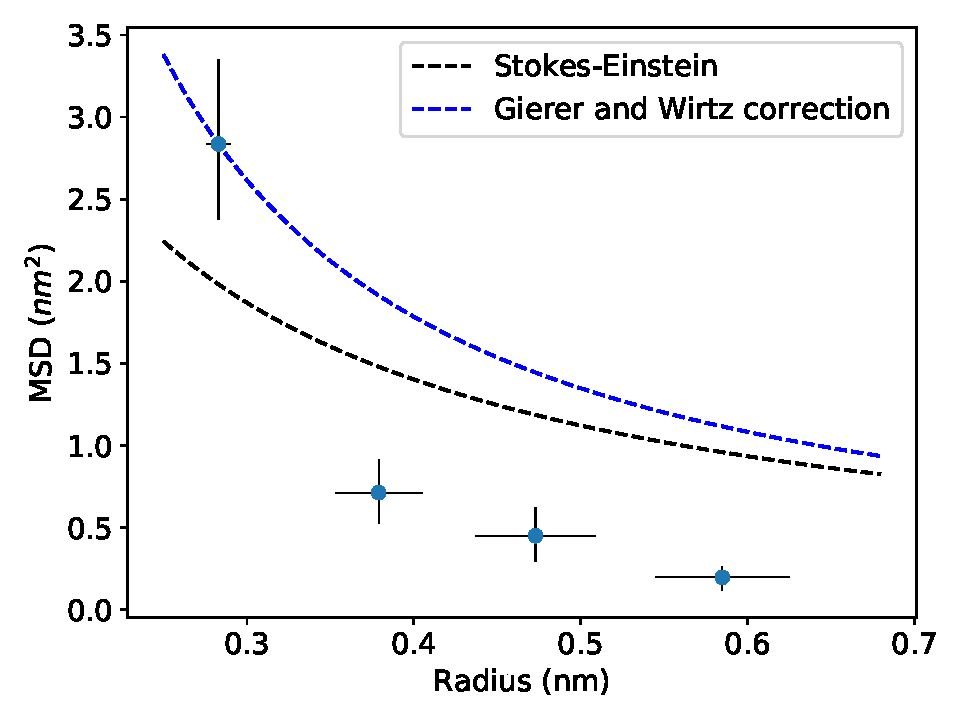
\includegraphics[width=\linewidth]{msd_radius_simple_alcohols_10wt.pdf}
  \caption{}\label{fig:msd_radius_simple_alcohol_rdf}
  \end{subfigure}
  \begin{subfigure}{0.45\textwidth}
  % BJC: update legends with abbreviations?
  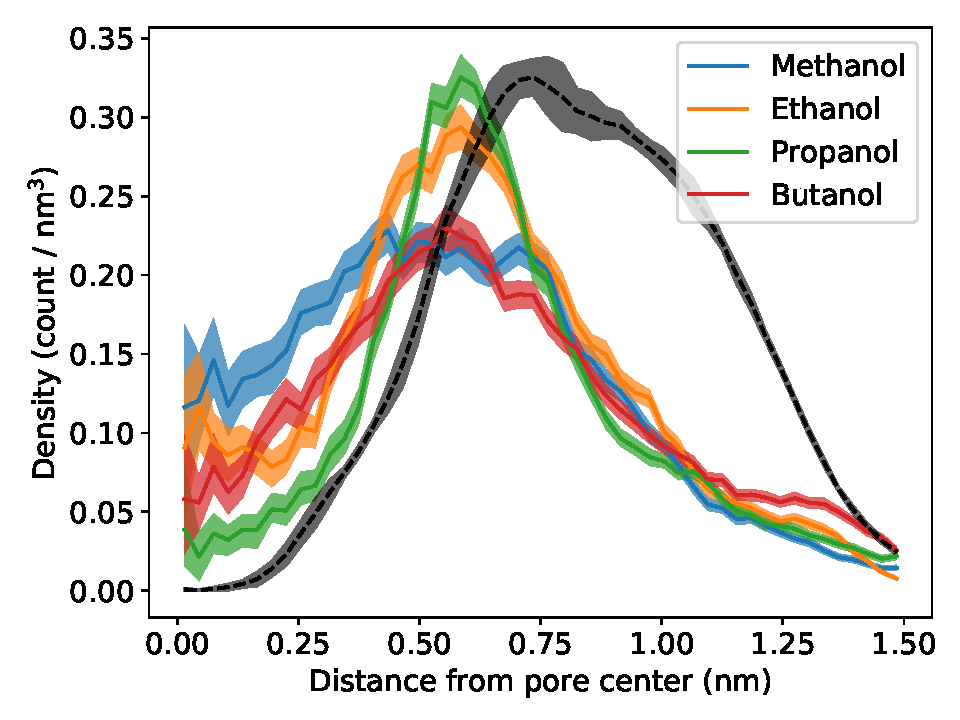
\includegraphics[width=\linewidth]{simple_alcohol_rdf.pdf}
  \caption{}\label{fig:simple_alcohol_rdf}
  \end{subfigure}
  \begin{subfigure}{0.45\textwidth}
  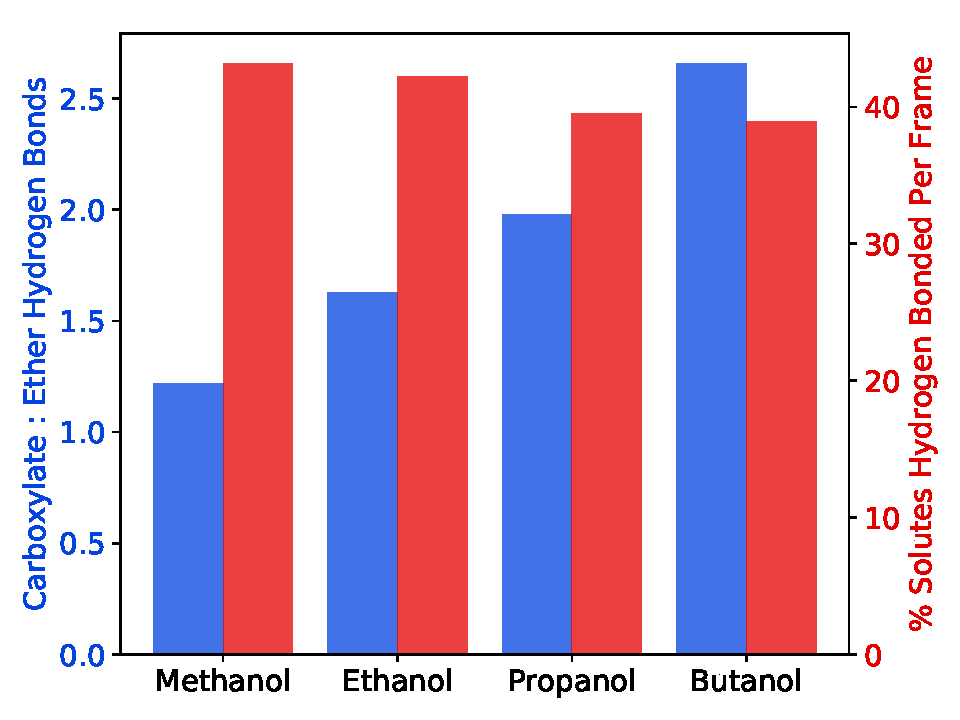
\includegraphics[width=\linewidth]{simple_alcohol_hbonds.pdf}
  \caption{}\label{fig:simple_alcohol_hbonds}
  \end{subfigure}
  \begin{subfigure}{0.45\textwidth}
  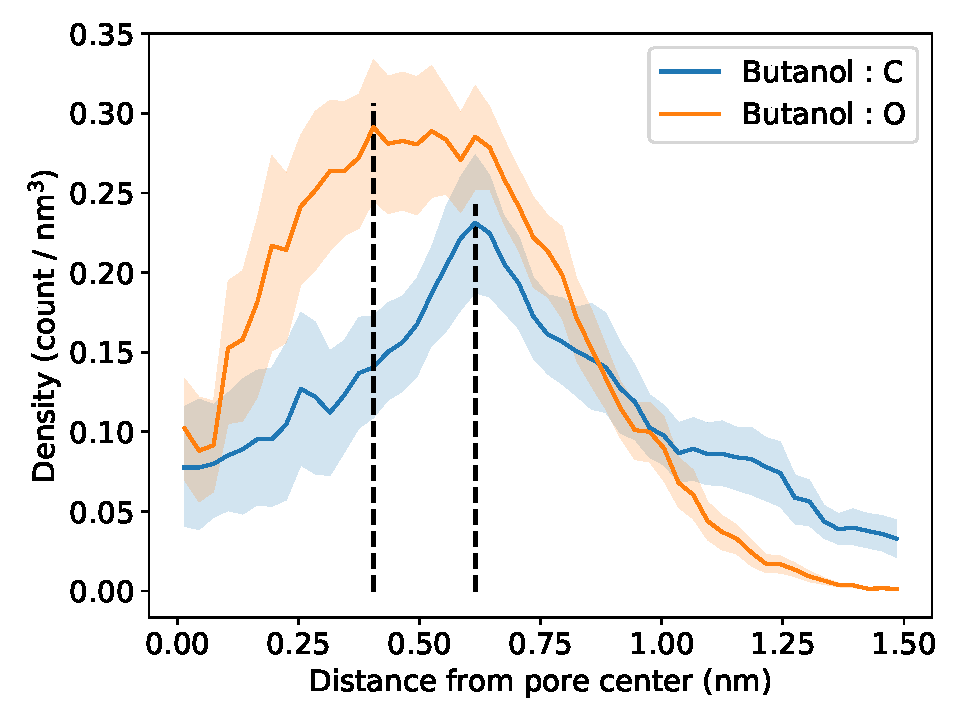
\includegraphics[width=\linewidth]{butanol_CO.pdf}\lapbox[\width]{-2.85cm}{\raisebox{3cm}{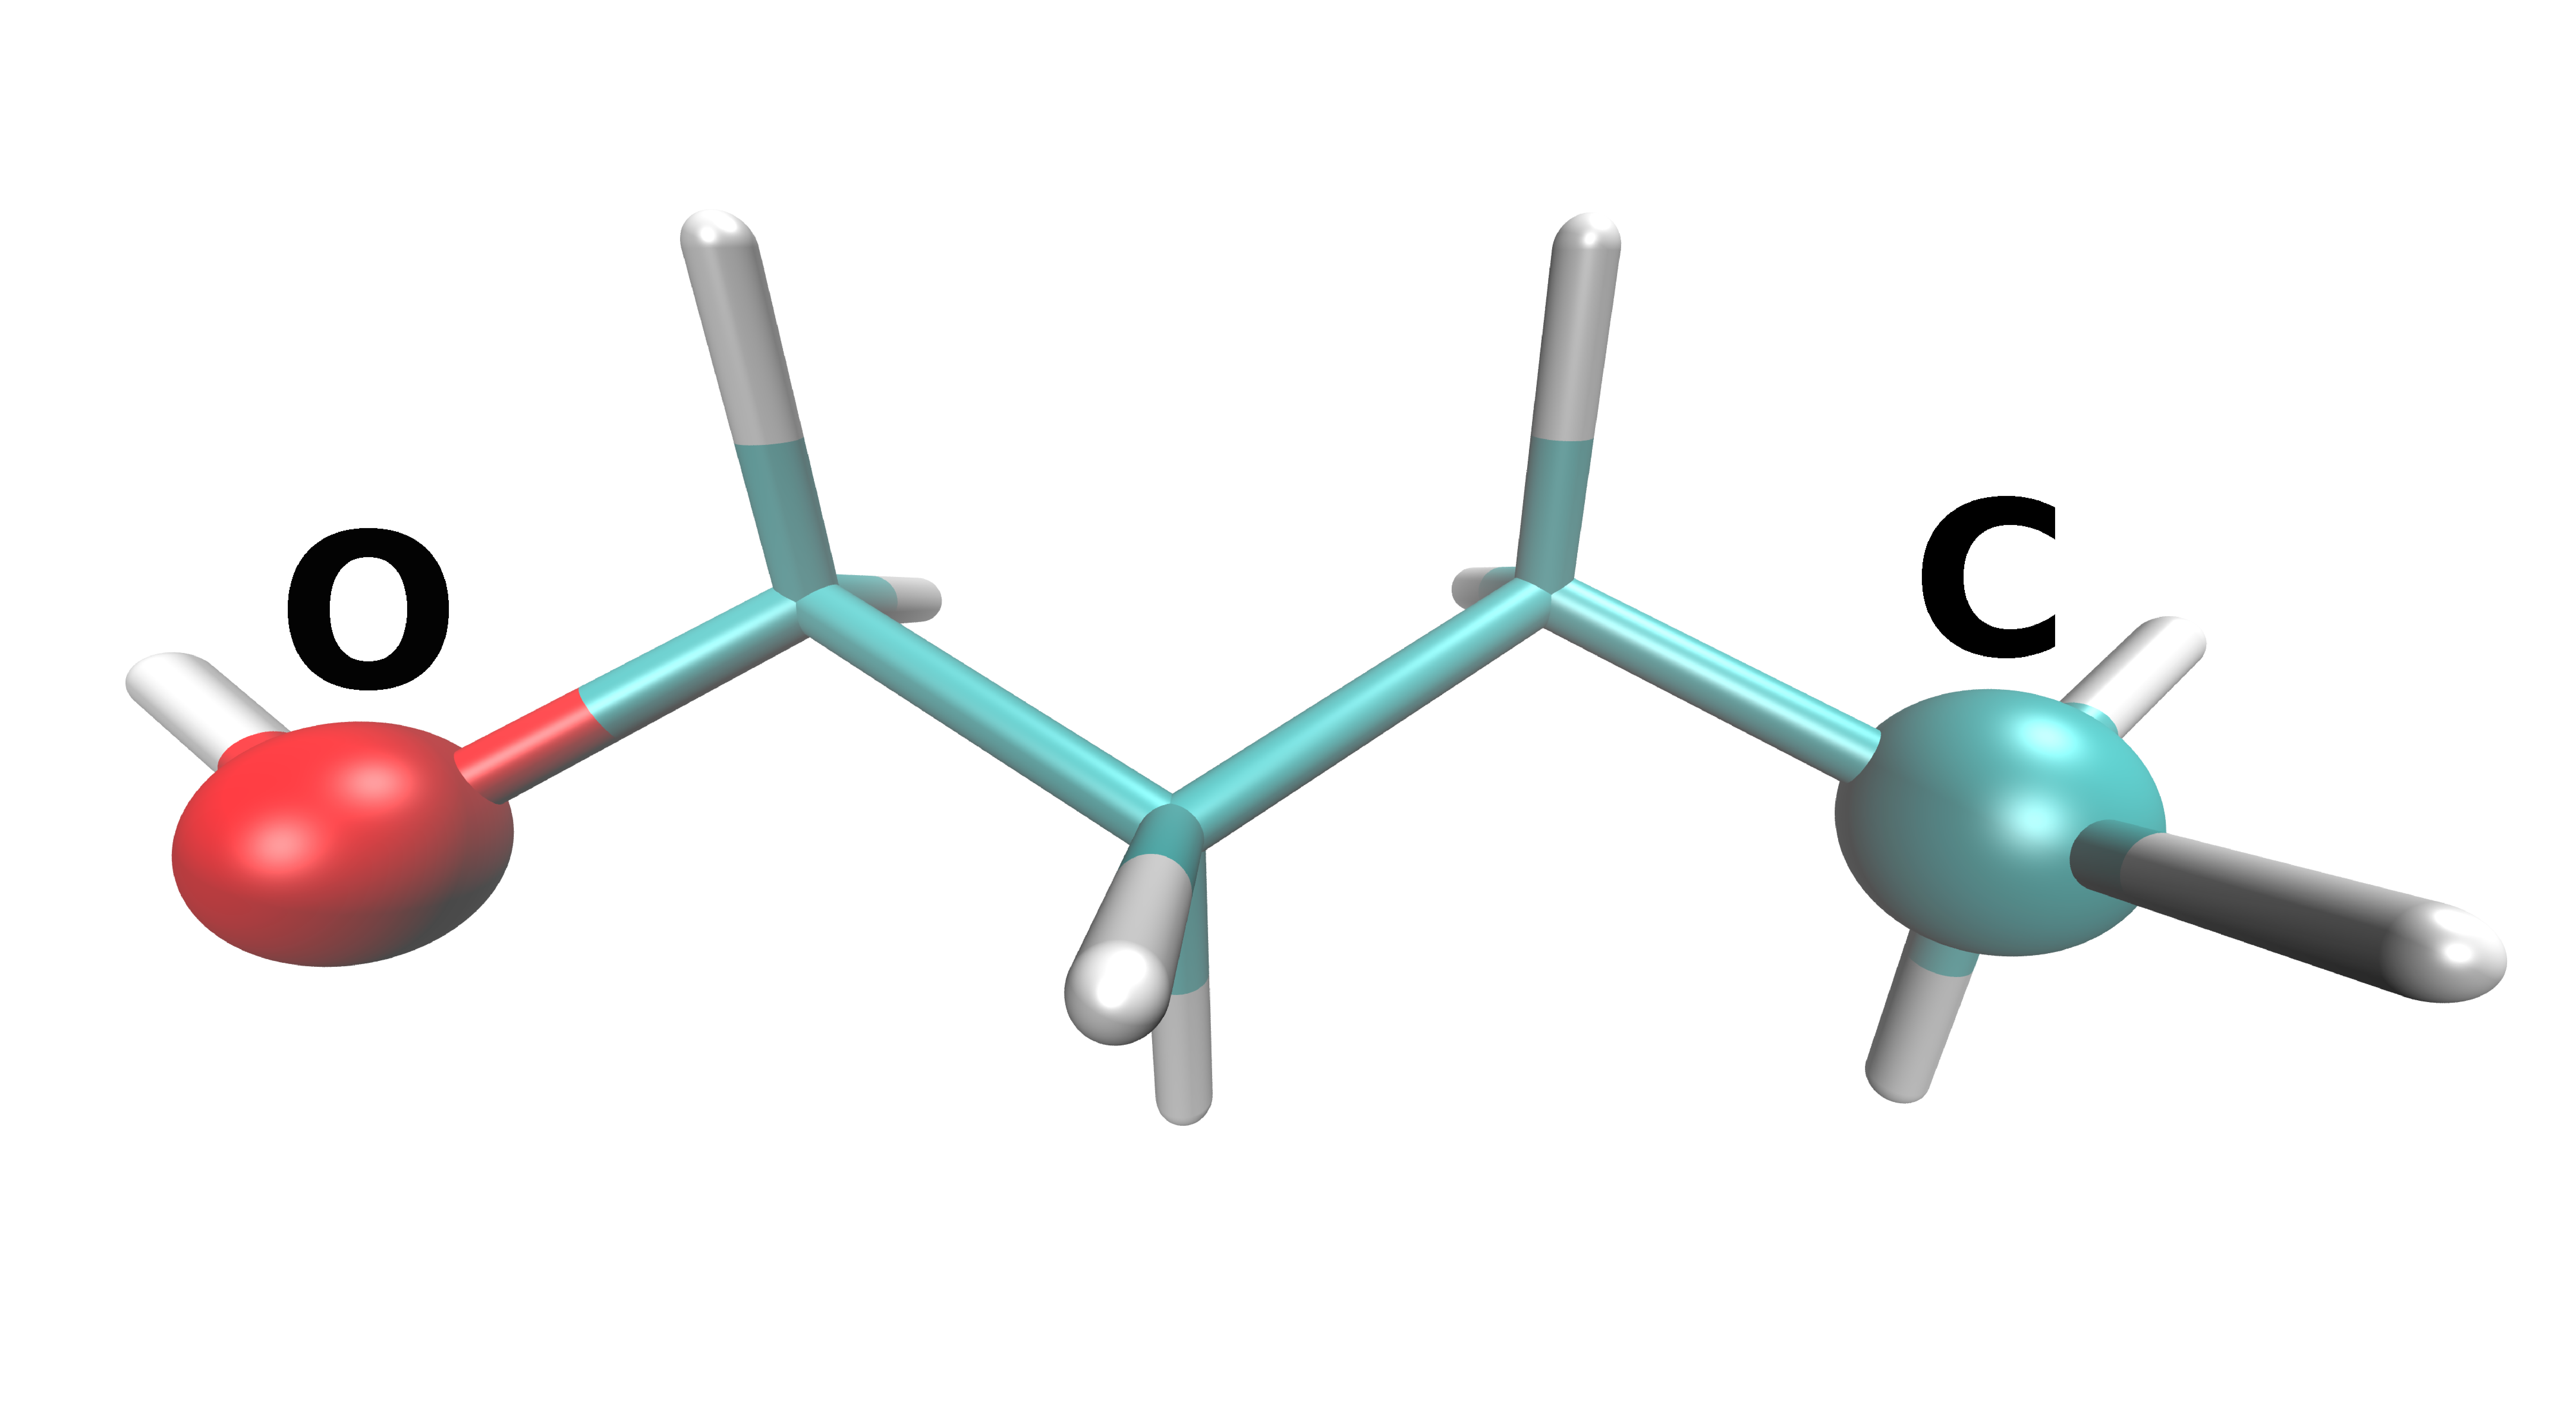
\includegraphics[height=1.4cm]{butanol_labeled.pdf}}}
  \caption{}\label{fig:butanol_CO}
  \end{subfigure}
  %MRS4: suggest putting something at the beginning of the caption indicating which chemical group it is.
  %BJC3: added to first sentence of caption
  \caption{(a) The MSD of the simple alcohols decrease as a function of the
  solute size, however the MSDs of ethanol, propanol and butanol are considerably
  lower than expected based on the Stokes-Einstein equation. (b) The radial 
  distribution functions of each simple alcohol shows a maximum close to the
  highest density of monomer head groups (normalized based on propanol's maximum
  density for easier visual comparison). Methanol spends the largest proportion 
  of time, relative to the other alcohols, near the pore center, which may help
  explain its fast dynamics. (c) Despite relatively little difference in the 
  total number of solutes actively participating in a hydrogen bond each frame,
  a given alcohol's preference towards hydrogen bonds with the carboxylate groups
  over ether linkages increases with increasing hydrophobic character. (d) The average location of 
  butanol's oxygen atom is closer to the pore center than its most distal carbon
  atom, suggesting that the molecule is oriented with hydrophobic tails pointing
  away from the pore center.}\label{fig:simple_alcohols}
  \end{figure}

  \subsection{Transport of Diols, Triols and Sugars}\label{section:polyols}
  
  The order of the MSDs of the diols, triols and sugars are roughly consistent with 
  their size; however, propylene glycol moves exceptionally slowly (see 
  Figure~\ref{fig:polyols_msd}). Ethylene glycol has the highest MSD followed
  by tetrose and glycerol, whose MSDs are similar, propylene glycol, the second
  smallest solute of this set, and finally ribose.
  
  Transport is both facilitated and hindered by additional solute hydroxyl groups
  due to their influence on radial density and hydrogen bond frequency. Extra 
  hydroxyl groups cause solutes to favor the water-rich pore region where there 
  is the least hindrance to movement (see Figure~\ref{fig:polyols_rdf}). Tetrose,
  ribose and glycerol are densest close to the pore center. They spend a greater
  fraction of their time in the pore region than any other solute (see 
  Figure~\ref{fig:frac_time}). This is likely a consequence of both their 
  hydrophilicity and large size which prevents them from partitioning into the 
  head group region. However, these extra hydroxyl groups facilitate a larger 
  number of hydrogen bond interactions that work to hold solutes in place (see 
  Figure~\ref{fig:multi_hbonds}). It has been observed that hydrogen bonding 
  in a system will generally reduce diffusivity.~\cite{srinivas_computer_1999}
  
  The number of hydrogen bonding interactions between solutes and head groups
  increases with the number of solute hydroxyl groups. These solutes frequently
  undergo simultaneous hydrogen bond interactions as shown in 
  Figure~\ref{fig:multi_hbonds}. For example, both hydroxyl groups of ethylene
  glycol can undergo hydrogen bonds with different hydrogen bond acceptors at 
  the same time. In some cases, all 4 hydroxyl groups of ribose hydrogen bond
  to monomer head groups simultaneously. As a consequence, hydrogen bond 
  lifetimes in these cases tend to be longer (see Figure~\ref{fig:hbond_dwells})
  since the solute positions are stabilized by multiple interactions. When one
  hydrogen bond is broken, the remaining unbroken hydrogen bonds keep the 
  molecule in place and allow the previously broken bond to reform.
%  Hydrogen bonds act as a kind of 
%  molecular glue which holds solutes in place, especially when there are many.
  Proximity to the pore center partially compensates for this effect in
  the cases of glycerol and tetrose, causing them to have relatively high MSDs
  for their size.
  
  \begin{figure}[!htb]
  \centering
  \begin{subfigure}{0.325\textwidth}
  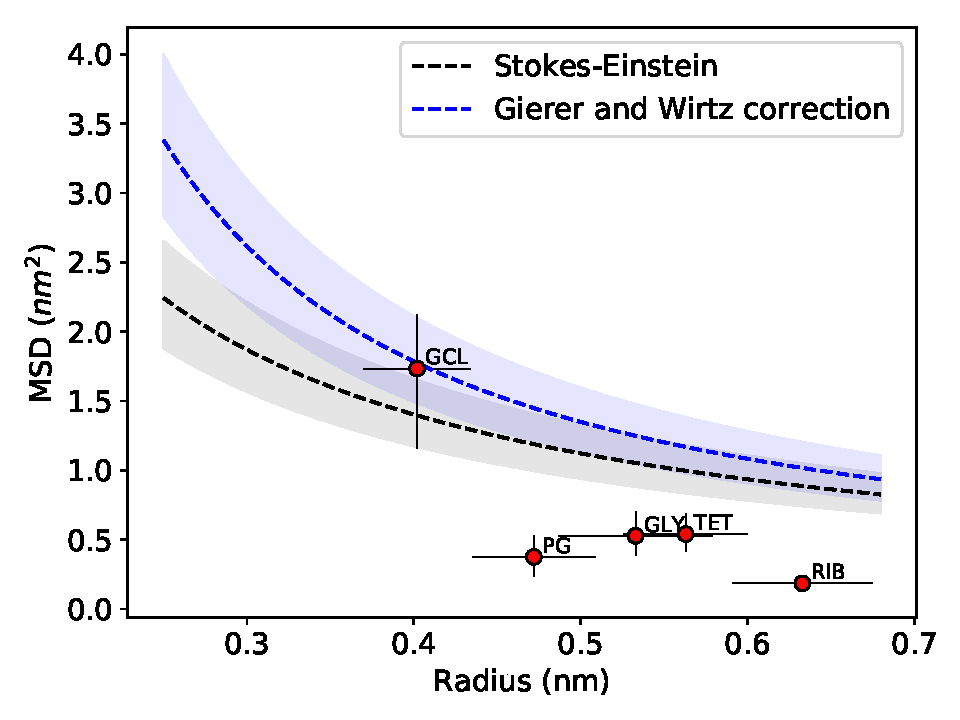
\includegraphics[width=\linewidth]{msd_radius_diols_10wt.pdf}
  \caption{}\label{fig:polyols_msd}
  \end{subfigure}
  \begin{subfigure}{0.325\textwidth}
  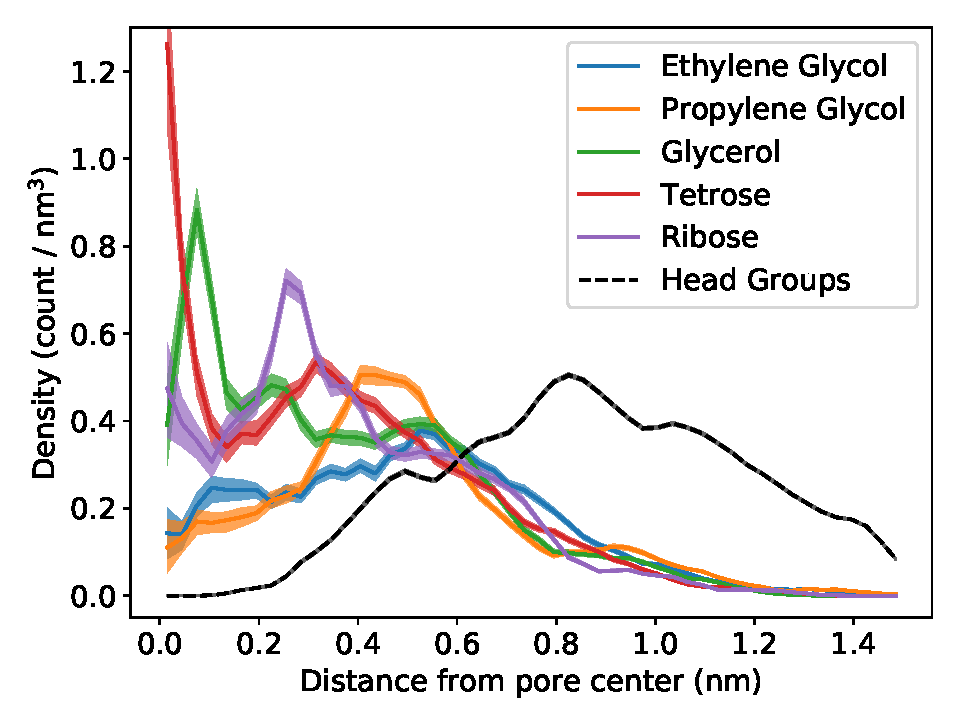
\includegraphics[width=\linewidth]{polyols_rdf.pdf}
  \caption{}\label{fig:polyols_rdf}
  \end{subfigure}
  \begin{subfigure}{0.325\textwidth}
  \vspace{-0.275cm}
  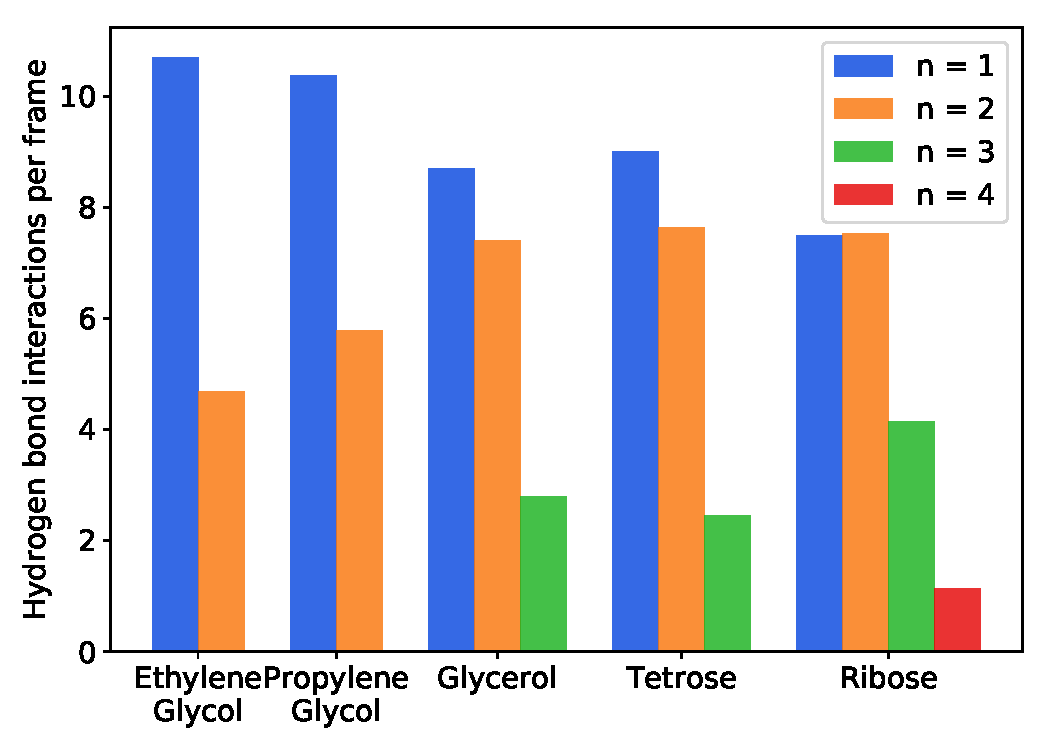
\includegraphics[width=\linewidth]{multi_hbonds.pdf}
  \caption{}\label{fig:multi_hbonds}
  \end{subfigure}
  \caption{(a) The MSDs of diols, triols and sugars descend in order of their size, except
  for propylene glycol which moves exceptionally slow. The MSD of ethylene glycol 
  is in close agreement with the theoretical lines, implying that the solute 
  is subject to a similar amount of hindrance as methanol, the solute to which the
  theoretical lines were fit. (b) Glycerol, tetrose and ribose have high densities 
  close to the pore center because they have a high number of hydrophilic groups and
  are relatively large. Ethylene glycol and propylene glycol are densest close to the
  head group region. (c) The number of hydrogen bond interactions between solutes and
  monomers increases as solutes gain additional hydroxyl groups. The number of 
  hydrogen bonds made by a single solute in different locations simultaneously, n, 
  also increases with the number of hydroxyl groups. In the most extreme case, all 
  four hydroxyl groups of Ribose (n = 4) are involved in a hydrogen bond interaction
  at the same time.}\label{fig:polyols}
  \end{figure}
  
  Of the two diols, ethylene glycol moves significantly faster than propylene
  glycol due to propylene glycol's affinity for the monomer head groups.
  Combined with an increase in size, the addition of a single methyl group to
  ethylene glycol increases propylene glycol's hydrophobic character and causes
  it to favor positions near monomer head groups (see Figure~\ref{fig:polyols_rdf}).
  Both diols have comparable densities close to the pore center, however propylene
  glycol's density has a large peak near the monomer head groups relative to 
  ethylene glycol. Propylene glycol can form more highly stabilized hydrogen 
  bonds with carboxylate groups, explaining the slightly higher incidence of 
  hydrogen bonds shown in Figure~\ref{fig:multi_hbonds}. The 95\textsuperscript{th}
  percentile of hydrogen bond lifetimes for propylene glycol with monomers is 
  9.5 ns compared to 7 ns for ethylene glycol. Somewhat counterintuitively, there is a 
  relatively high density of ethylene glycol molecules beyond the head group region
  probably due to its relatively small size. This likely contributes to the somewhat
  large error bars on its MSD in Figure~\ref{fig:msds}. 

  \subsection{Transport of Ketones and Amides}
  
  The 4 ketone-like molecules tested show a range of transport behaviors. 
  Urea, acetic acid, acetamide and acetone are all characterized by
  a carbonyl group with two attached heavy atoms. All are similar in size and
  are planar molecules due to the $sp^2$ hybridization of their carbonyl group. 
  The fastest solutes of this grouping, acetic acid and urea, move about 3
  times faster than the slowest, acetone.
  
  The amides, urea and acetamide, hydrogen bond with head groups relatively 
  infrequently, but regularly coordinate with sodium ions (see 
  Figure~\ref{fig:ketones}). In an average frame, over 50\% of acetic acid molecules
  participate in hydrogen bonds with monomer head groups while less than 
  10\% of urea and acetamide molecules hydrogen bond with head groups. 
  Urea and acetamide both have hydrogen bond donating nitrogen atoms, however
  nitrogen is a weaker hydrogen bond donor than oxygen due to its lower 
  electronegativity.~\cite{biswal_hydrogen_2015} Given their lower propensity
  to hydrogen bond, one might expect amides to partition out of the pore 
  and/or to move through the pore quickly, perhaps faster than methanol. 
  However, both RDFs contain sharp peaks situated between the pore center
  and the head groups, but closer to the pore center than other solutes 
  that hydrogen bond with carboxylate groups. Solutes that
  hydrogen bond frequently tend to show peaks in their RDFs near 0.5-0.6 nm 
  from the pore center (see Figure~\ref{fig:simple_alcohol_rdf}, for example)
  and those that coordinate with sodium ions more frequently tend to show 
  peaks in their RDFs near 0.2-0.4 nm from the pore center. Both solutes spend
  about half of their time with their carbonyl oxygen atom coordinated to a
  sodium ion which restrains the solutes to within the pore region
  
  Among the solutes in this set, only the carbonyl oxygen atoms coordinate 
  with sodium ions. The nitrogen atoms do not coordinate at all despite a
  similar negative partial charge because the attached hydrogen atoms 
  shield this interaction by making the NH\textsubscript{2} group 
  approximately neutral.

  Acetone has the lowest MSD of this set because it either coordinates with
  sodium or stays trapped near and behind the head groups. Acetone spends the
  smallest fraction of time in the pore region out of all solutes in this study
  (see Figure~\ref{fig:frac_time}). On average, acetone coordinates with sodium
  with the same frequency as acetic acid which is manifested as a peak in its 
  RDF about 0.2 nm from the pore center. 
%  However, acetic acid spends 
%  significantly more time in the pore center and therefore encounters more sodium ions. 
  %When an acetone molecule coordinates with a sodium ion, its polarity is
  %largely neutralized and it retreats towards the head group region where it can easily
  %get trapped. 
  Acetic acid and the amides have other, unoccupied, hydrophilic groups while
  bound to sodium ions which increases their stability in the pore.
  
  \begin{figure}[!htb]
  \centering
  \begin{subfigure}{0.325\textwidth}
  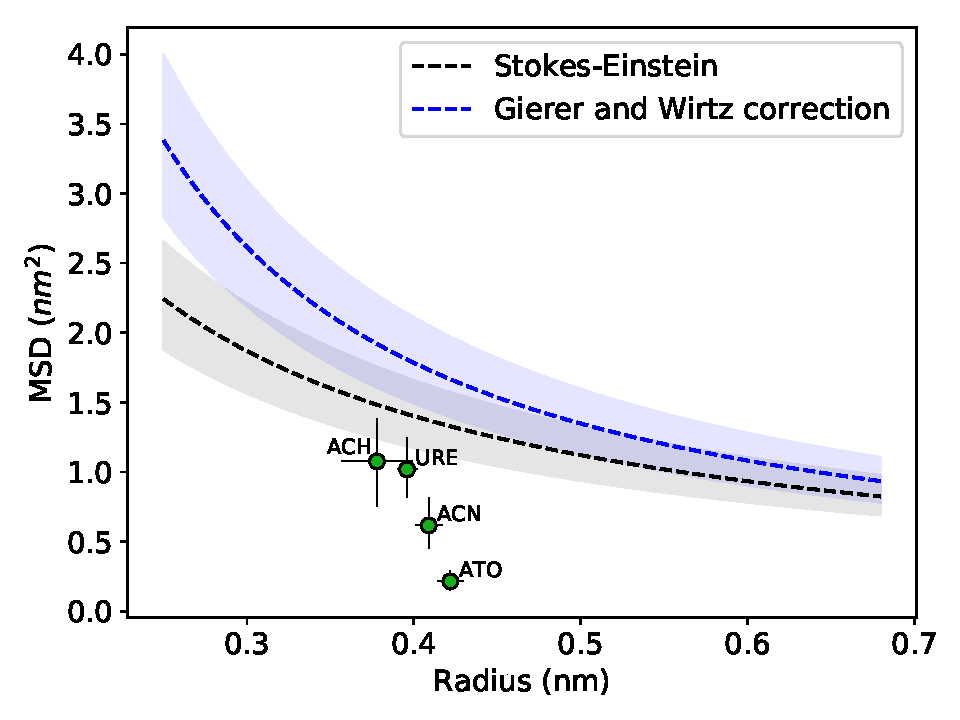
\includegraphics[width=\textwidth]{msd_radius_ketones_10wt.pdf}
  \caption{}\label{fig:ketones_rdf}
  \end{subfigure}
  \begin{subfigure}{0.325\textwidth}
  \includegraphics[width=\textwidth]{ketone_rdf.pdf}
  \caption{}\label{fig:ketones_rdf}
  \end{subfigure}
  \begin{subfigure}{0.325\textwidth}
  \includegraphics[width=\textwidth]{ketone_hbonds.pdf}
  \caption{}\label{fig:ketone_hbonds}
  \end{subfigure}
  \caption{(a) The MSD of ketones and amides decreases and the deviation from
  Stokes-Einstein predicted behavior increases with molecular size.
  (b) The radial density near the pore center (r = 0) decreases with decreasing
  solute MSD. Peaks in the RDFs of urea, acetamide and acetone that appear 
  0.2 - 0.4 nm from the pore center are likely due to coordination with sodium
  ions. (c) The amides hydrogen bond with water far less than acetic acid, 
  however they tend to coordinate with sodium ions more frequently. Acetone
  coordinates with sodium with same frequency as acetic acid.}\label{fig:ketones}
  \end{figure}
  
  \subsection{Transport of Thiols}
  
  We also studied the transport properties of sulfur analogs of glycerol,
  ethylene glycol and acetone. We replaced all but one oxygen atom of 
  ethylene glycol and glycerol with sulfur atoms to create dimercaptoethanol
  and 2,3-dimercapto-1-propanol. We replaced the carbonyl carbon of acetone
  with sulfur in order to create DMSO. Sulfur-containing compounds form weaker
  hydrogen bonds than nitrogen and oxygen-containing compounds due to their
  low electronegativity.~\cite{biswal_hydrogen_2015} For this reason, thiols
  are less soluble in water than their hydroxyl group analogs.
  
  \begin{figure}[!htb]
  \centering
  \begin{subfigure}{0.45\linewidth}
  %BJC: should I plot ethylene glycol, glycerol and acetone MSDs here as well?
  \includegraphics[width=\textwidth]{msd_radius_sulfur_10wt.pdf}
  \caption{}\label{fig:msd_radius_sulfur_10wt}
  \end{subfigure}
  \begin{subfigure}{0.45\linewidth}
  \includegraphics[width=\textwidth]{thiol_comparison_SOH.pdf}
  \caption{}\label{fig:SOH_GCL_comparison}
  \end{subfigure}
  \begin{subfigure}{0.45\linewidth}
  \includegraphics[width=\textwidth]{thiol_comparison_DMP.pdf}
  \caption{}\label{fig:DMP_GLY_comparison}
  \end{subfigure}
  \begin{subfigure}{0.45\linewidth}
  \includegraphics[width=\textwidth]{thiol_comparison_DMS.pdf}
  \caption{}\label{fig:DMS_ATO_comparison}
  \end{subfigure}
  \caption{(a) The RDF of mercaptoethanol is similar to ethylene glycol except 
  for its higher density in the tail region and consequently lower density in the
  pore region. (b) 2,3-dimercapto-1-propanol is densest near the head groups, 
  unlike glycerol whose density is very high close to the pore center. 
  (c) Overall, dimethylsulfoxide has a higher density than acetone within the 
  pore region which may in part explain its marginally larger MSD.}\label{fig:sulfur_analog_rdfs}
  \end{figure}
  
  Mercaptoethanol has a similar average MSD and RDF to ethylene glycol
  (see Figures~\ref{fig:all_msds_10wt} and~\ref{fig:SOH_GCL_comparison}).
  There is a much larger uncertainty associated with mercaptoethanol's
  MSD. The range of behaviors shown by mercaptoethanol help explain the
  large variance of its MSD. Much can be accounted for by the higher 
  density of mercaptoethanol molecules outside the pore region, where 
  transport is inherently slower. Although both solutes
  hop with a similar magnitude inside and outside of the pore region, mercaptoethanol 
  spends about 18\% less time in the pore region (see Figure~\ref{fig:hops}).
  This has a large impact on its hop frequency which is 42\% lower than that 
  of ethylene glycol. This implies that mercaptoethanol is relatively
  immobile outside of the pore, but moves quickly inside.
%  Mercaptoethanol also hydrogen bonds with head groups about 16\% less 
%  %BJC: 16\% less meaning 64.3 % - 48.3 %. Not sure if it is better to say (64.3 - 48.3 / 64.3) = 25 %
%  frequently. Consequently, shorter hydrogen 
%  bond lifetimes within the pore region may yield some high MSD 
%  trajectories. 

%, which is less than expected if equal amounts of both 
%  solutes occupied the pore region. 
% (20.2 - 12.857) / 20.2 = .364
% (12.857 + 6.8215 + 0.803) / (20.2 + 11.969 + 1.935) = 0.6
%  There are nearly 40\% more mercaptoethanol 
%  molecules than ethylene glycol molecules beyond 0.8 nm  % ratios.py in figures folder
%  from the pore center. 
%  The average length
%  of a hop performed by a mercaptoethanol molecule within 0.8 nm of the pore 
%  center is 1.43 nm compared to 1.20 for ethylene glycol. % hop_location.py. Even larger difference if cut-off lower
  
  2,3-dimercapto-1-propanol exhibits slower transport than glycerol 
  because more of it partitions into the tail region (see 
  Figure~\ref{fig:DMP_GLY_comparison}). 2,3-dimercapto-1-propanol
  spends 27\% less time in the pore region than glycerol. 
  %BJC: again, not sure if this should be 27\% because DMP spends 49% of time in pore and GLY spends 76% of time in pore or if it should be (76 - 49) / 76 = 36 %
%  The density of glycerol is always higher up to 0.7 nm from the pore center where the 
%  population of 2,3-dimercapto-1-propanol then becomes more dense into the tail region.
  Glycerol participates in about 2.5 times as many hydrogen
  bonds as 2,3-dimercapto-1-propanol (including all possible hydrogen bonding groups).  % BJC: might be confusing. Maybe refer to figure 6 instead.
  % BJC: sums are (donate to monomer + receive from water + donate to water).
  % BJC: (31.91 + 17.224 + 3.231) / (13.1 + 7.737 + 0.8965) ~= 2.45.
  % (2.788 + 2.0975 + 0)/ (13.1 + 7.737 + 0.8965) = 0.22
  Only 22\% of the hydrogen bond interactions of 2,3-dimercapto-1-propanol
  involve sulfur. Because sulfur can only weakly hydrogen bond, 
  2,3-dimercapto-1-propanol is less soluble than glycerol in the water-filled
  pores and more readily partitions into the tail region.
  
  DMSO has a comparable MSD to acetone even though it is a larger molecule
  (see Figure~\ref{fig:msds}). DMSO spends 17\% more time in the pore than acetone. 
%  The density of DMSO is higher than acetone in the pore region, except for
%  the peak exhibited by acetone near 0.2 nm, which is due to sodium ion association.
  On average, 35\% of DMSO molecules are coordinated to a sodium ion each
  frame compared with 26\% of acetone molecules. The pyramidal structure 
  of DMSO may force it to spend more time closer to the pore center which
  increases its interaction with sodium ions. The tendency of DMSO to stay
  in the pore region counterbalances the sodium ion interactions to give it
  a higher MSD than acetone. 
  
  \subsection{Solutes Unable to Donate Hydrogen Bonds}  % Need a better heading since all molecules in this study are acceptors

  The slowest set of molecules we studied can accept hydrogen bonds, but
  cannot donate them. Among this set are the two slowest solutes in our study: 
  THF and DMF. The MSDs of ethyl acetate, propylene carbonate and acetone are
  only marginally larger.
  
  The solutes in this set have small hop lengths. 3 of the bottom 6 mean hop
  lengths are associated with ethyl acetate, propylene carbonate and
  dimethyl formamide (Figure~\ref{fig:hop_lengths}). Acetone and 
  tetrahydrofuran perform slightly larger hops but with low hop frequencies
  (see Figure~\ref{fig:hopfreq}).
  
  The radial density of solutes near the pore center in this set is 
  surprisingly high as shown in Figure~\ref{fig:nondonors_rdf}. Propylene
  carbonate and ethyl acetate are among the largest solutes in this study. 
  Their size prevents them from easily entering the tail region and 
  consequently leads to faster transport properties.  % since they spend more time in the pore region. 
  However, this is not a hard rule. When a solute does overcome the 
  barrier of entry beyond the pore region, it can become trapped. All
  solutes in this set show at least a small peak in the pore region which
  is caused by solutes that get trapped in the tail region for 
  significant periods of time.
    
%  The solutes in this set do not make frequent hops while in the pore region. 
%  % Time bound to sodium ion
%  % Number of hops in pore region
%  \begin{itemize}
%%	\item Observations of single THF trajectories have revealed that it becomes 
%%	nearly immobilized while associated with sodium ions 
%%	(See Figure~\ref{fig:thf_sodium_coordination}).
%	\item DMF experiences a similar effect, but to a lesser extent. Its density is 
%	higher than THF near the head groups. The planar shape of DMF causes it to 
%	become stuck between head groups. Excursions into the pore region do not
%	necessarily result in large hops.
%  \end{itemize}
  
  Carbonyl groups continue to show high degrees of association with
  sodium ions. Between 25 and 30\% of propylene carbonate, dimethyl 
  formamide and ethyl acetate molecules are coordinated with sodium ions
  for a given frame which is consistent with the coordination exhibited by acetone
  (see Figure~\ref{fig:nondonors_hbonds}). The carbonyl group of the amides 
  studied in the previous section associate with sodium nearly twice as 
  frequently as compounds that don't contain nitrogen 
  (see Figure~\ref{fig:ketone_hbonds}).
  Association between sodium and solutes in this set are also among the longest,
  only beaten by other solutes with carbonyl groups and ribose.
 
  \begin{figure}[!htb]
  \centering
  \begin{subfigure}{0.325\textwidth}
  \includegraphics[width=\textwidth]{msd_radius_nondonors_10wt.pdf}
  \caption{}\label{fig:nondonors_rdf}
  \end{subfigure}
  \begin{subfigure}{0.325\textwidth}
  %BJC: trying out pore region cut-off here instead of head groups.
  \includegraphics[width=\textwidth]{nondonors_rdf.pdf}
  \caption{}\label{fig:nondonors_rdf}
  \end{subfigure}
  \begin{subfigure}{0.325\textwidth}
  \includegraphics[width=\textwidth]{nondonor_hbonds.pdf}
  \caption{}\label{fig:nondonors_hbonds}
  \end{subfigure}
  \caption{(a) The MSDs of solutes that can only receive hydrogen bonds are
  significantly lower than expected. (b) The solutes' radial density
  is surprisingly high in the pore region, but is balanced by an appreciable
  amount of solute trapped in the tails. (c) The low MSDs exhibited by each of these
  solutes is due to a combination of entrapment within the tail region and a high 
  degree of coordination with sodium ions.}\label{fig:nondonors}
  \end{figure}

  \section{Conclusion}

  We have examined the transport characteristics of a series of small polar
  molecules in our model of the H\textsubscript{II} phase formed by the liquid 
  crystal monomer Na-GA3C11. We found that transport of solutes is 
  %MRS3: tweak
  %primarily
  governed by both water content as well as the interplay between the chemical functionality of the solute
  and the chemical functionality of the LLC monomer and ion making up the pore. 
  We 
  %MRS3:
  have shown
  that the MSD of solutes, water and counter ions are highly 
  dependent on LLC membrane water content. As more water is added to the system, 
  the pores become 
  %less crowded with monomer components. 
  more dilute in the monomer components.
  The MSDs of water and
  sodium ions are nearly 2 orders of magnitude larger in the 10 wt\% system 
  than in the 5 wt\% system. The amount of water in the pores 
  %MRS3:
  thus
  deserves special
  attention when screening new monomers.
  
  The transport of polar solutes in this system is significantly slower than
  that of water due to their interaction with the LLC monomers. We observed 
  three primary mechanisms of solute entrapment within the pores.
  \begin{enumerate}
    \item Solutes can become entangled among monomer tails. 
    \item Solutes can donate hydrogen bonds to immobile monomers.
    \item Solutes can associate with counterions.
  \end{enumerate}
  
  The chemical functionality of solutes influences the degree to which
  they are affected by each trapping mechanism. Simple alcohols tend to
  partition into the tail region as their hydrophobic tail increases in length.
  Alcohols and sugars with multiple hydroxyl groups are very stable
  in the pore region, but 
  %frequent 
  multiple
  hydrogen bonds with monomer head 
  groups prevent them from diffusing quickly. This effect is reduced when
  hydroxyl groups are replaced with thiol groups, but the solutes become less
  stable in the pore. Finally, solutes with carbonyl groups, which includes
  the ketones, amides and solutes that can only accept hydrogen bonds, associate
  with sodium ions, temporarily slowing or immobilizing them. 

  %MRS2: trying something else to emphasize what we are trying to do.  Can you add a bit more detail so it's not just slowing up or speeding solutes, but slowing or speeding up solutes of a particular type?  We can emphasize chemical selectivity . . . 
  %mitigate or enhance their effect on   solute MSDs.   
  %BJC3: gave it a try. Broke into paragraphs
  Based on these trapping mechanisms, we may be able to suggest modifications
  that can be made to monomers that will modulate their effect on specific 
  solute MSDs in order to make transport even more selective for particular 
  solutes. 
  %MRS3: I'd actually suggest connecting these; since above is a thesis statement for the next bit. 
  Since solutes move slowly while entangled among the monomer tails,
  and since more than half of the solutes studied spend at least 40\% of their
  time in the tails, one can try to design monomers that better control the 
  partition of solutes between the pore and tail region. Solutes move into 
  the tails due both to their size and hydrophilic character. One may be 
  able to contain solutes, even small ones like methanol, by increasing
  the density of monomers close to the head groups through incorporation of 
  cross-linkable groups in the vicinity. Alternatively, removal of the ether
  linkages between the head groups and the monomer tails may decrease the 
  stability of any of the molecules we studied near the head groups and 
  force them to spend more time within the pore. 
  
  %Solutes that spend a large fraction of their 
  %time in the tails, such as butanol with its high hydrophilic character, could
  %exhibit higher permeabilities from these types of changes. 
  
  One could instead focus on designing head groups with varying hydrogen bonding
  capabilities. Increasing the number of hydrogen bonding sites on the head 
  groups may enhance the membrane's ability to trap solutes like sugars that 
  have multiple hydroxyl groups. Conversely, one can decrease the number of hydrogen
  bonding sites, or replace them with weaker hydrogen bonding atoms like nitrogen, to
  trap less. In contrast to the system studied here, one can design the head 
  groups so they can donate hydrogen bonds, which can enhance entrapment of 
  solutes like acetone that can only accept hydrogen bonds.
  
  Finally, one can attempt to control the degree to which solutes coordinate
  with counterions. Increasing the valence of the counterions may cause them
  to bind more strongly to solutes which may be a useful way to trap 
  carbonyl-containing solutes like urea for longer periods of time. Of course,
  an increased valence would require proportionately less total counter ions
  to balance the system charge which could result in the opposite effect. One
  could also design the head groups so that counterions are negatively charged
  which may eliminate their interaction with most solutes.
 
%  
%  These hypotheses remain to be tested in future simulations of new
%  monomers.
  
  The findings here are likely too complex to point towards a clear design of an 
  optimal LLC membrane for a particular separation. This work does demonstrate
  that there is a large range of solute-membrane interactions resulting from the
  chemically complex and inhomogeneous LLC membrane structure. The varying 
  chemical functionality of the solutes themselves gives rise to an immense diversity of
  transport behavior. This behavior suggests that a large range of chemical 
  selectivities may be possible in self-assembled nanoporous membranes. Atomistic
  modeling gives us the opportunity to observe these interactions at the molecular
  scale, at least approximately, so that we can think more critically about 
  nanostructured membrane design. 

  \section*{Supporting Information}

  Detailed explanations and expansions upon the results and procedures mentioned in
  the main text are described in the Supporting Information. This information is
  available free of charge via the Internet at http://pubs.acs.org.

  \section*{Acknowledgments}

  Molecular simulations were performed using the Extreme Science and
  Engineering Discovery Environment (XSEDE), which is supported by National
  Science Foundation (NSF) grant number ACI-1548562. Specifically, it used the Bridges
  system, which is supported by NSF award number ACI-1445606, at the Pittsburgh
  Supercomputing Center (PSC). This work also utilized the RMACC Summit supercomputer,
  which is supported by the NSF (awards ACI-1532235 and
  ACI-1532236), the University of Colorado Boulder, and Colorado State
  University. The Summit supercomputer is a joint effort of the University of
  Colorado Boulder and Colorado State University.
  
  The authors thank Christopher Calderon and Gregory Morrin for helping kick start
  our studies of subdiffusive transport. Additionally, the authors thank 
  Douglas Gin and Richard Noble for their guidance on past and present experimental
  research on LLC membranes and for reading over this manuscript before submission.

  \clearpage

  \bibliographystyle{ieeetr}
  \bibliography{transport}

  \newpage

  \section*{TOC Graphic}
  
  \begin{figure}[!htb]
  \centering
  \includegraphics[width=3.25in]{toc_transport.pdf}
  \end{figure}

\end{document}

% LocalWords:  lyotropic LLC solutes solute permeability micropollutants RO NF
% LocalWords:  groundwaters flowback nanofiltration bruggen Nanostructured feng
% LocalWords:  nanostructured mesophases Donnan Zhou al Dischinger BJC Hmm Na
% LocalWords:  selectivities physicochemical nanopores GA pKa's protonated pKa
% LocalWords:  gallic perrin pka NaGA MeOH URE EtOH acetamide AcN propanol PrOH
% LocalWords:  butanol BtOH mercaptoethanol EG sulfoxide DMSO PG dimercapto DMP
% LocalWords:  GLY tetrahydrofuran THF tetrose dimethylformamide DMF AcOH diols
% LocalWords:  triols MSD solute's readthedocs repo GROMACS gromacs der hess wt
% LocalWords:  Antechamber bccsym molcharge QUACPAC zhou Resel equil ca gmx COM
% LocalWords:  solvate solvated Parrinello barostat subdiffusive superdiffusive
% LocalWords:  subdiffusion CTRW MSDs ageing microfriction Gierer einstein Chan
% LocalWords:  MSD's comps li Rg appoximation polson bT fr CI Luzar Chandler py
% LocalWords:  hbonds VMD Roux genion disassociated Clauset martiniano Voloshin
% LocalWords:  timescales binned RDFs RDF tortuosity carboxylate pdf sodium's
% LocalWords:  mobilities timescale diffusivity msd tailvpore methanol's tamsds
% LocalWords:  msds sublinear ztraces COMs alkane COOH HOH hbond immobilization
% LocalWords:  counterions sulfinyl substituents electronegative COH coord na
% LocalWords:  Carvajal Wu Shinoda carboxy ATPase rdf counterintuitively Amides
% LocalWords:  unhindered propanol's butanol's hydrophilicity glycol's Ketones
% LocalWords:  hybridization amides electronegativity NH ketones Thiols SOH ACI
% LocalWords:  dimercaptoethanol dimethylsulfoxide rdfs mercaptoethanol's thiol
% LocalWords:  formamide nondonors nanoporous XSEDE PSC RMACC TET ribose EAC
% LocalWords:  berendsen spoel Rahman bulleted Wirtz TBD equilibrations thiols
% LocalWords:  hbonding DMS linkable permeabilities Calderon Morrin TOC
